\documentclass[12pt]{article}

% Page geometry
\usepackage[right=1.25in,left=1.25in,top=1.1in,bottom=1.1in]{geometry}

% Fonts and input
\usepackage[T1]{fontenc}
\usepackage[utf8]{inputenc}
\usepackage[english]{babel}

% Math
\usepackage{amsmath,amsthm,amsfonts,amssymb,bm}

% Figures and tables
\usepackage{graphicx}
\usepackage[section]{placeins}
\usepackage{caption}
\usepackage{subcaption}   % <-- modern subfigure package
\usepackage{threeparttable}
\usepackage{multirow}
\usepackage{tabularx,ragged2e,booktabs}
\usepackage{array}

% Bibliography
\usepackage[natbibapa]{apacite}
\bibliographystyle{apacite}
\setcitestyle{aysep={}}

% Formatting
\usepackage{color}
\usepackage{setspace}
\usepackage[export]{adjustbox}
\usepackage{titlesec}
\usepackage[title]{appendix}
\usepackage{ulem}      % for \normalem
\normalem
\usepackage{sectsty}
\usepackage{comment}
\usepackage{footmisc}
\usepackage{pdflscape}

% Hyperlinks
\usepackage{hyperref}
\hypersetup{
  colorlinks,
  citecolor=blue,
  filecolor=blue,
  linkcolor=blue,
  urlcolor=blue
}

% Colors
\definecolor{darkgreen}{rgb}{0.0,0.7,0.0}

% Line spacing
\onehalfspacing

% Theorems
\newtheorem*{definition}{Definition} 
\newtheorem{assumption}{Assumption} 
\newtheorem{proposition}{Proposition} 
\newtheorem*{lemma}{Lemma} 
\newtheorem{theorem}{Theorem}
\newtheorem{corollary}[theorem]{Corollary}
\newtheorem{hyp}{Hypothesis}
\newtheorem{subhyp}{Hypothesis}[hyp]
\renewcommand{\thesubhyp}{\thehyp\alph{subhyp}}

% Math operators
\DeclareMathOperator*{\argmax}{argmax} 

% Custom commands
\newcommand{\red}[1]{{\color{red} #1}}
\newcommand{\blue}[1]{{\color{blue} #1}}

% Column types
\newcolumntype{L}[1]{>{\raggedright\let\newline\\arraybackslash\hspace{0pt}}m{#1}}
\newcolumntype{C}[1]{>{\centering\let\newline\\arraybackslash\hspace{0pt}}m{#1}}
\newcolumntype{R}[1]{>{\raggedleft\let\newline\\arraybackslash\hspace{0pt}}m{#1}}

% Special table cell
\newcommand{\specialcell}[2][c]{\begin{tabular}[#1]{@{}l@{}}#2\end{tabular}}

\begin{document}

\begin{titlepage}
\title{Joint calibration of the volatility surface and variance term structure}
\author{Jiwook Yoo\thanks{Any views expressed in this article are solely those of the author. I thank David Hsieh for his comments and feedback on many prior drafts of this article. I also extend thanks more broadly to the finance faculty at the Fuqua School of Business for their helpful comments. All errors are my own. For email correspondence: \href{mailto:jiwook.yoo@duke.edu}{jiwook.yoo@duke.edu}. }}
\date{\today}
\maketitle
\vspace{-1.5em}

\begin{abstract}
\noindent This article proposes a calibration framework for complex option pricing models that jointly fits market option prices and the term structure of variance. Calibrated models under the conventional objective function, the sum of squared errors in Black–Scholes implied volatilities, can produce model-implied variance term structures with large errors relative to those observed in the market and implied by option prices. I show that this can occur even when the model-implied volatility surface closely matches the volatility surface observed in the market. The proposed joint calibration addresses this issue by augmenting the conventional objective function with a penalty term for large deviations from the observed variance term structure. This augmented objective function features a hyperparameter that governs the relative weight placed on the volatility surface and the variance term structure. I test this framework on a jump-diffusion model with stochastic volatility in two calibration exercises: the first using volatility surfaces generated under a Bates model, and the second using a panel of S\&P 500 equity index options covering the 1996–2023 period. I demonstrate that the proposed method is able to fit observed option prices well while delivering realistic term structures of variance. Finally, I provide guidance on the choice of hyperparameters based on the results of these numerical exercises.  \\
\vspace{0in}\\
\noindent\textbf{Keywords:} Model calibration, volatility surface, variance term structure \\
\noindent\textbf{JEL Codes:} C52, G13, G17\\

\bigskip
\end{abstract}
\setcounter{page}{0}
\thispagestyle{empty}
\end{titlepage}
\pagebreak \newpage


\section{Introduction}
Parametric option pricing models are workhorses of contemporary academic research and industry practice. At a high level, the selection of a particular model is to specify the stochastic process for the underlying asset's price as well as for any other relevant state variables, with the parameters of these processes often calibrated to closely match observed market prices. The distribution implied by these processes in turn informs a risk-neutral measure from which derivative prices and hedge ratios are derived. This workflow has its roots in the classic works of \cite{black1973pricing} and \cite{black1976pricing} who model an underlying asset as a geometric Brownian motion (GBM) and calibrate the GBM diffusive variance to fit option prices. However, a large body of evidence suggests that asset prices exhibit time series properties that differ from a simple GBM. Asset prices can jump \citep{carr2002fine, bollerslev2011tails}, possess time-varying volatility \citep{shephard2005stochastic}, exhibit a leverage effect \citep{carr2017leverage}, and deviate in a myriad of other ways not captured by a simple drift-diffusion process. In response, researchers and industry practitioners alike have considered more complex models that aim to shore up deficiencies by more faithfully modeling these underlying processes (e.g. adding jumps, stochastic volatility, etc). However, these more sophisticated models are more difficult to calibrate and can produce models with unrealistic implications \citep{cont2004nonparametric}. One of these implications which are at odds with the data is the economically unrealistic term structure of variance these models imply. The purpose of this article is to propose a general model calibration framework which can calibrate complex models that produce realistic term structures of variance while still closely matching observed option prices.

Broadly speaking, the calibration of an option pricing model involves minimizing some function of the model fitting error to search for the a set of parameters which minimizes this error, thereby producing the best fit. Generally, the function being minimized is a weighted sum of squared errors, either in terms of prices or implied volatilities. Particularly for complex models, it is well-known that the problem of minimizing such an objective function can be ill-posed, resulting in a range of issues related to numerical implementation  \citep{cont2003financial}. For instance, the objective function may not be globally convex or might possess very flat regions. In such cases, the numerical optimization procedure used to minimize the objective function may fail to converge to a minimum. Even when this procedure does converge, the resulting set of parameters can imply economically unreasonable implications such as large derivations from the variance term structure observed in the market. This can pose a significant problem for academic work that relies on the calibration of such models to study the pricing of variance and its associated risk premia. 

At the core of my framework is the variance term structure implied by option prices. It is well-known that the term structure of variance is pinned down by option prices although this identification is complicated in the case that the underlying can jump. If the underlying price process is continuous, \cite{neuberger1994log} and \cite{dupire1994pricing} provide a model-free construction of the risk-neutral expected variance of the underlying asset $S_t$ over any time horizon $[t,t+\tau]$. This expected variance can be identified provided there are European-style options on the underlying expiring at time $t+\tau$. If the underlying can jump, the pricing of variance is more subtle. Recent work by \cite{carr2021pricing} and \cite{carr2021robust} shows how to precisely recover the risk-neutral expected variance under very general settings. However, unlike in the continuous case, this replication is no longer model-independent; rather, it depends on the higher-order moments of the jump distribution. My proposed calibration procedure uses the information in the variance term structure to directly augment a standard objective function used for calibrating option pricing models, the sum of squared errors in option implied volatilities. 

To fix ideas, let $\sigma^{mkt}(K_{i,j}, \tau_j)$ be the Black-Scholes implied volatility (BSIV) of an out-of-the-money (OTM) European-style option with strike price $K_{i,j}$ and maturity $\tau_j$ obtained by inverting the option's observed price.\footnote{For this article, I consider a strike price $K$ and to be out-of-the-money if $K \geq S$ for call options and $K < S$ for put options where $S$ is the spot price of the underlying.} Let $\sigma^{mod}(K_{i,j}, \tau_j;  \Theta)$ denote the model implied BSIV where the model parameters are stored in the vector $\Theta$. Like for the market BSIVs, I invert the model-implied price via the \cite{black1973pricing} formula. The standard objective function minimized in calibration is given in \eqref{eq: std_obj}:
\begin{equation}\label{eq: std_obj}
    \sum\limits_{j}\sum\limits_{i} w_{i,j}\left[\sigma^{mod}(K_{i,j}, \tau_i; \Theta) - \sigma^{mkt}(K_{i,j}, \tau_j)\right]^2 
\end{equation}
where $w_{i,j}$ are non-negative weights. The main idea of my approach uses the variance term structure to augment this objective function with an additional term which penalizes deviations from the variance term structure observed in the market. Let $V^{mkt}(\tau)$ be the variance implied by market option prices and $V^{mod}(\tau; \Theta)$ be the model-implied variance with parameter vector $\Theta$.\footnote{To match market conventions for quoting variance, I work with all variance quantities in terms of annualized variance.} The augmented objective function I propose has the following general form:
\begin{equation}\label{eq: obj_fun}
    \alpha \left(\sum\limits_j\sum\limits_{i} w_{i,j}\left[\sigma^{mod}(K_{i,j}, \tau_j; \Theta) - \sigma^{mkt}(K_{i,j}, \tau_j)\right]^2\right)  + (1-\alpha) \left(\sum\limits_{j} y_j \left[\sqrt{V^{mod}(\tau; \Theta)} - \sqrt{V^{mkt}(\tau)}\right]^2\right) 
\end{equation}
where $w_i$ and $\tau_j$ are non-negative weights. The right-most sum in \eqref{eq: obj_fun} is taken over all observed maturities $\tau$ rather than over individual contracts $i$ as is the case in the first sum. For the purposes of consistency and considering "like" quantities across the two summations, the second sum considers the error in the implied volatilities rather than variances. The constant $\alpha \in [0,1]$ is a hyper-parameter which governs the trade-off between fitting the option implied volatilities and fitting the term structure of implied variance. When the objective function in \eqref{eq: obj_fun} is used to calibrate option pricing models, the behavior of the calibrated model may sharply differ depending on the value of $\alpha$. At the extremes, an $\alpha$ of one purely emphasizes matching market BSIVs across contracts while an $\alpha$ equal to zero directs the model to solely fit the term structure of variance. 

The closest approach in spirit to my proposed methodology found in the literature  is that of \cite{andersen2015parametric}. They propose a similar objective function which also directly augments the standard sum in squared errors of option implied volatilities with a penalization term. Rather than penalizing errors in the term structure of variance, their objective function penalizes deviations of the model's spot diffusive variance from a non-parametric estimate of diffusive variance. Other approaches to calibration incorporate information from variance, either under risk-neutral or physical measure, in a variety of ways. For instance, \cite{pan2002jump}, \cite{ait2002maximum}, \cite{ait2020term}, among many others utilize information from the term structure of variance to simultaneously calibrate option pricing models and identify risk premia.  Of more thematic relation is the vast literature that seeks to reconcile the pricing of SPX (S\&P 500) options with the term structure of the VIX or the pricing of the various derivatives based on it (i.e. VIX index options, VIX futures, etc). For example, \cite{jacquier2018vix} show how to use VIX futures to calibrate a rough Bergomi model to SPX options. Another example is the two-factor option pricing model of \cite{zhao2013unifying}, which he calibrates using the term structure of the VIX and the prices of index options written on SPX and VIX. 

The rest of this article discusses the calibration of option pricing models using an objective function with the functional form in \eqref{eq: obj_fun}. The first half of section \ref{sec: theory} gives an overview of the theoretical setting, known results, and a discussion of related literature. In the latter half, I provide motivation and theoretical results related to my proposed objective function. Section \ref{sec: data} describes the panel of S\&P 500 options used in my empirical analysis and gives an overview of time series properties of the variance term structure implied by those options. Section \ref{subsec: simulations} is an analysis of the calibration procedure on simulated option data. In section \ref{subsec: SPX_fit}, I apply my proposed methodology to the stochastic volatility, jump-diffusion model of \cite{bates1996jumps} to fit index options on SPX and examine model implications for the jump distribution in \eqref{subsec: SPX_jump_process}. Lastly, section \ref{sec: conclusion} concludes and proposes various use cases and best practices.


\section{Theory and related literature}\label{sec: theory}
I motivate my results in continuous time with mild restrictions on the underlying stochastic processes. I postulate the a general set of risk-neutral dynamics for the underlying $S_t$ consisting of a diffusive term and a jump component that arrives according to a Poisson process: 
\begin{equation}\label{eq: general_process}
d S_t=\left(r-\lambda \mu_J\right) S_t d t+\sqrt{V_t} S_t d W_t+\left[\exp(J_t)-1\right] S_t d N_t     \qquad  \mathbb{P}(dN_t = 1) = \lambda dt
\end{equation}
where $r$ is the risk-free rate and $\lambda \mu_J$ is the compensator for the predictable component of the jump process. I impose the following conditions on the process: (1) the variance process $V_t$ has finite long-run mean, and (2) that the first two moments of $J_t$, its mean $\mu_J$ and variance $\sigma_J^2$, exist. The stochastic process in equation \eqref{eq: general_process} nests many familiar price processes featured in parametric option pricing models. Examples include the \cite{black1973pricing} model, the \cite{hull1990pricing} stochastic volatility model, and the \cite{bates1996jumps} model which pairs stochastic volatility with the jump process from the \cite{merton1976option} model.

In continuous time, the realized variance of a price process is measured by the quadratic variation of its log price. For the price process in \eqref{eq: general_process}, the quadratic variation from time 0 to $\tau$, $QV(\tau)$, is given by:
\begin{equation}\label{eq: QV}
 QV(\tau) = \int_0^{\tau} \left(d\log S_t\right)^2 =   \left(\int_0^{\tau}  V_t d t + \int_0^{\tau}  \int_{\mathbb{R}} J^2 \nu(d s, d x)\right)
\end{equation}
where $\nu(d s, d x)$ is the jump product measure. Traded derivatives based on variance, most notably variance swaps, use a function of annualized quadratic variation as the payoff.\footnote{In practice, the payoff of these derivatives discretize the integrals in \eqref{eq: QV} often approximating the continuous quadratic variation by the sum of squared log returns. See \cite{bondarenko2014variance} for a detailed overview and analysis of this discretized payoff. } I adopt this market convention here and annualize all measures of variance in this article. Given a model with parameter vector $\Theta$ informing the stochastic process in \eqref{eq: general_process}, one can compute the annualized expected variance from time $0$ to $\tau$ under the model-implied distribution. For ease of exposition, I refer to this quantity as $VS(\tau\vert \Theta)$, the variance swap rate for maturity $\tau$ computed under the model with parameters $\Theta$. I compute $VS(\tau)$ in equation \eqref{eq: imp_var} below where $\mathbb{E}_0(\cdot\vert \Theta)$ denotes the expectation operator with respect to the model-implied pricing measure $\mathbb{Q}_\Theta$:
\begin{equation}\label{eq: imp_var}
 VS(\tau; \Theta) = \dfrac{1}{\tau}  \mathbb{E}_0^{mod}\left[QV(\tau) \vert \Theta\right] = \dfrac{1}{\tau} \mathbb{E}_0\left[\int_0^{\tau} V_t  d t + \int_0^{\tau} \int_{\mathbb{R}} J^2 \nu(d s, d x)\right]
\end{equation}
The terminology and convention comes from the market for variance swaps. For the purposes of this paper, I refer to quantities like $VS(\tau; \Theta)$, based on expected quadratic variation like in \eqref{eq: imp_var}, as the price of a variance swap with maturity $\tau$. In practice, variance swaps have zero price at initiation and pay a single payoff at maturity to holder of the long position equal to the difference between the annualized realized variance $QV(\tau)$ over the swap's life and $VS(\tau\vert \Theta)$. This difference is multiplied by some notional value which just scales up the variance swap payoff:
$$\left[QV(\tau) - VS(\tau\vert \Theta) \right] \times \text{Notional}$$
Such instruments allow for market participants to hedge variance directly or otherwise express a view about the market pricing of variance. Note it is only when realized variance from time $0$ to $\tau$, $QV(\tau)$, is unexpectedly higher than what was expected at time $0$ (under the model-implied risk neutral distribution) that payoff is positive. Many modern asset pricing models posit a negative variance risk premium in equity markets. Empirical studies lend support to this view, with studies of synthesized and market variance swap quotes suggesting, on average, the payoff of these swaps are negative \citep{carr2009variance, konstantinidi2016does}. 

A related quantity is the highly-referenced VIX Index maintained by the Chicago Board of Exchange (CBOE). The VIX Index, more accurately its square, is constructed via a static replication method and is proportional to the price of the so-called log contract \citep{neuberger1994log}. For simplicity of notation, I define the log contract with maturity $\tau$ here as the claim which pays $-\log(S_{\tau}/S_0)$ at time $\tau$ where $S_t$ is the time $t$ price of the underlying.  Since the log contract is a European-style claim, one can recover the VIX by pricing the log contract from vanilla options by applying the well-known payoff spanning results of \cite{breeden1978prices} and \cite{carr1998towards}.\footnote{For a function $g: [0,\infty]\to \mathbb{R}$ with continuous second derivative, the time 0 price of a European-style contingent claim paying $g(S_T)$ at maturing at time $T$ is equal to the price of a portfolio of options given by $g(S_0) + \int_0^F g''(K)P_0(K) \, dK +  \int_F^\infty g''(K)C_0(K) \, dK $ where $F$ denotes the forward price. The log contract is priced by setting $g(K) = -\log(K)$.} Let $C_0(K, \tau)$ and $P_0(K, \tau)$ be the time 0 prices of call and put contracts respectively. I define the quantity $VIX^2(\tau)$ to be
\begin{equation}\label{eq: VIX}
    VIX^2(\tau) = 2 \mathbb{E}^\mathbb{Q}\left[-\dfrac{1}{\tau}\log\dfrac{S_\tau}{S_0}\right] = 2\left[\dfrac{1}{\tau}\int_0^{F_\tau} \dfrac{P_0(K,\tau)}{K^2} \, dK + \dfrac{1}{\tau} \int_{F_\tau}^\infty \dfrac{C_0(K,\tau)}{K^2}  \, dK \right]
\end{equation}
where $F_\tau$ is the $\tau$ forward price of the index at time 0 and $\mathbb{E}^\mathbb{Q}$ is the expectation operator over the market pricing measure $\mathbb{Q}$. Setting $\tau$ equal to 1/12 (one month maturity) and taking the square root delivers the VIX Index reported by CBOE. 

% shore up this portion
In practice, one cannot simply compute the value of the integrals such as those appearing in equation \eqref{eq: VIX_cont} as it would require observing a continuum of strike prices. To compute such integrals, I implement the standard discretization approach ubiquitous to both the literature and industry practice. Suppose we only observe put and call prices for the increasing sequence of strike prices $\lbrace K_j\rbrace_{j=1}^{N_\tau}$ with time to maturity $\tau$ where $N_\tau$ is the number observed strikes. To approximate an integral with integrand of form $g(K)C_0(K,\tau)$ for a generic function $g(K)$, I discretize the integral using the following approximation:
\begin{equation}\label{eq: disc}
  \int_{0}^{\infty} g(K)C_0(K, \tau) \, dK  \approx   \sum\limits_{j=1}^{N_\tau } g(K)C_0(K, \tau)\Delta(K_j)
\end{equation}
The sum in \eqref{eq: disc} is taken over all strikes in $\lbrace K_j\rbrace_{j=1}^{N_\tau }$. $\Delta(K_j)$ is given by:
\begin{equation}
    \Delta(K_j) = \begin{cases}
K_2 - K_1 & \text{if }j = 1 \\
\dfrac{K_{j+1} - K_{j-1}}{2}   & \text{if } 1 < j < N_\tau \\
K_{N_\tau } - K_{N_\tau -1} & \text{if } j = N_\tau 
\end{cases}
\end{equation} 
I use an analogous computation for integrals with integrands of form $h(K)P_0(K,\tau)$. In order to compute the integrals in the VIX computation using $\eqref{eq: disc}$, one can set $g(K)$ to $\textbf{1}_{F_\tau \geq K}K^{-2}$ and $g(K)$ to $\textbf{1}_{F_\tau \leq K}K^{-2}$ for the first and second integrals on the right-hand side of equation \eqref{eq: VIX} respectively.\footnote{$\textbf{1}_{F_\tau \geq K}$ and $\textbf{1}_{F_\tau \leq K}$ are indicator functions for if the strike $K$ is OTM for puts and calls respectively.} 

The aim of the rest of this section is to provide a self-contained theoretical basis for my proposed calibration procedure for option pricing models based on observed option BSIVs and the term structure of variance. Section \ref{subsec: related_lit} discusses the existing approaches to calibrating option pricing models. Section \ref{subsec: vs}, gives an overview of the general theory of pricing variance swaps beginning with the continuous price process case then discussing the case where prices may jump. In sections \ref{subsubsec: theory_SJD} and \ref{subsubsec: theory_general}, I produce theoretical results which provide the motivation and basis for my proposed calibration methodology.


\subsection{Related literature: Calibration approaches and jump processes}\label{subsec: related_lit}
In both finance practice and the academic literature, calibrating a parametric option pricing model is a routine procedure. Systematic approaches to model calibration involve searching for parameters which best fit observed market prices or implied volatilities by some criterion. Early work, such as the study of \cite{amin1994implied} on Eurodollar options and futures, minimized the sum of squared errors in option prices to calibrate the interest rate model of \cite{heath1992bond}. \cite{bakshi1997empirical} compare calibration results from minimizing objective functions based on a sum of squared errors in both option prices and implied volatilities. For my own approach, minimizing a sum of squared BSIVs weighting all contracts equally serves as a starting point and valuable reference against which other objective functions can be compared. We can obtain this from the expression in \eqref{eq: std_obj}, setting $w_{i,j} = 1$ for all contracts:
\begin{equation}\label{eq: iv_sum}
   \sum\limits_{j} \sum\limits_{i} \left[\sigma^{mod}(K_{i,j}, \tau_j; \Theta) - \sigma^{mkt}(K_{i,j}, \tau_j)\right]^2 
\end{equation}
The sum in \eqref{eq: iv_sum} is taken over all OTM options observed in the market with strike prices given by $K_{i,j}$ and maturity by $\tau_j$. A popular alternative to using \eqref{eq: iv_sum} outright is to approximate the difference in implied volatilities using option prices and \cite{black1973pricing} vegas (e.g. \cite{christoffersen2009shape}).\footnote{This is the well-known "vega-weighting" approximation to \eqref{eq: iv_sum}. This approximation substitutes a first-order Taylor polynomial in the BSIV to approximate $\sigma^{mod}(K_i, \tau_i\vert \Theta) - \sigma^{mkt}(K_i, \tau_i)$ for each contract. } 

Related to the standard approach of minimizing squared errors is the more general approach of using moment conditions using the general method of moments framework introduced by \cite{hansen1982generalized}. \cite{chernov2000study} calibrate a discrete time stochastic volatility model using moments computed from the time series of underlying returns and option prices.  \cite{pan2002jump} expands on this approach, estimating a continuous time jump-diffusion model using moments from the physical measure and option-implied moments to recover risk premia associated with jumps. \cite{broadie2007model} consider a similar type of joint estimation using moments from physical and risk-neutral measures and investigate the effects of model mis-specification on inferred volatility and jump risk premia. 

Another class of approaches, which includes my own proposed methodology, makes use of a regularization term to the usual sum of squared errors in BSIVs or option prices. Denote by $P^{mkt}(K_i, \tau_i)$ and $P^{mod}(K_i, \tau_i; \Theta) $ the prices of an OTM option $i$ with strike $K_i$ and time to maturity $\tau_i$ observed in the market and under a model with parameters $\Theta$ respectively. The general forms of these objective functions are shown in \eqref{eq: obj_reg_prices} and \eqref{eq: obj_reg_ivs}:

\begin{equation}\label{eq: obj_reg_prices}
       \sum\limits_j \sum\limits_{i} w_{i,j}\left[P^{mod}(K_i, \tau_i ; \Theta) - P^{mkt}(K_i, \tau_i)\right]^2 + h(\Lambda; \Theta)
\end{equation}
\begin{equation}\label{eq: obj_reg_ivs}
       \sum\limits_j   \sum\limits_{i} w_{i,j}\left[\sigma^{mod}(K_i, \tau_i; \Theta) - \sigma^{mkt}(K_i, \tau_i)\right]^2 + h(\Lambda;\Theta)
\end{equation}
where $\Lambda$ denotes the regularization parameters and $h(\Lambda;\Theta)$ the regularization term. As discussed in detail in \cite{cont2003financial}, the inverse problem of calibration can be ill-posed or susceptible to issues related to numerical optimization. Intuitively, the motivation behind regularization aims to modify the objective function to have a desirable mathematical property (e.g. convexity, more curvature) in order to render it more amenable to numerical optimization. 

For example, \cite{cont2004nonparametric} propose a regularization term which is a function of relative entropy with respect to a prior pricing measure. Specifically, the authors suggest setting the penalization term $g(\Lambda; \Theta)$ in \eqref{eq: obj_reg_prices} and \eqref{eq: obj_reg_ivs} to $cD(\mathbb{Q}_\Theta, \mathbb{P}_0)$ where $D$ is the Kullback-Leibler (KL) divergence between the model-implied pricing measure $\mathbb{Q}_\Theta$ with respect to some prior measure $\mathbb{P}_0$.\footnote{$c$ is a scalar parameter which regulates the relative importance between KL penalization term and the standard sum of squares objective function.} \cite{lagnado1997technique} suggest an objective function as in \eqref{eq: obj_reg_prices} with a Tikhonov regularization term for $h(\Lambda; \Theta)$. This regularization term is a function of $\Vert \Theta - \Theta_0\Vert$ where $\Theta_0$ is some prior set of model parameters with sensible properties and $\Vert \cdot \Vert$ is an appropriately chosen vector norm. In the context of a local volatility model of the volatility surface, \cite{egger2005tikhonov} demonstrate stable convergence of Tikhonov regularization and provide recommendations for the choice of norm motivated by theoretical results. My own proposed objective function can be seen as an instance of \eqref{eq: obj_reg_ivs} where the regularization term is a function of deviations from the market observed variance swap or VIX term structures. The closest approach in the literature to my own is \cite{andersen2015parametric}, who utilize deviations from model-implied diffusive variance and observed diffusive variance estimated from high frequency price quotes to regularize a standard sum of squared errors in BSIVs.

Lastly, some methodologies propose exploiting asymptotic formulas for implied volatility at long-dated maturities or at extremely OTM strikes to either inform a choice of starting values or to select a subset of parameters outright. Choosing a subset of parameters prior to numerical calibration increases computational efficiency due to the reduction in dimensionality of the optimization problem featured in calibration. For instance, the moment formula of \cite{lee2004option} can be used to infer the two parameters of the \cite{kou2002jump} jump-diffusion model. \cite{forde2010asymptotic} derive asymptotic formulas for implied volatility in the context of the Heston model which provide a closed-form approximation of the implied volatility function, allowing for quick calibration on an approximated Heston model. The parameters recovered from calibration on the approximated model in turn can provide informative starting values for calibration on the exact model. 

\subsection{Identification of variance term structure}\label{subsec: vs}
Throughout the 1990s, developments by \cite{neuberger1994log}, \cite{dupire1994pricing}, \cite{carr1998towards} and \cite{demeterfi1999} provided the theoretical basis for the valuation of contracts based on the quantity in \eqref{eq: imp_var}. In light of these theoretical developments, CBOE in 2003 switched over to a "model-free" calculation of the VIX from their prior methodology based on at-the-money Black-Scholes implied volatility.\cite{carr2012variance}, the VIX is based on the static replication methodology of obtaining fair strike of a variance swap; this replication is model-free as long as price process of the underlying asset is continuous. If the process can jump, the (positive) negative skewness of the jump distribution biases the replication downwards (upwards).  Over the 2000s, a number of tradable instruments were introduced to meet the growing demand to trade and hedge variance and volatility risk. In 2004, CBOE introduced VIX futures and followed up with European-style index options written on the VIX in 2006. Today, the valuation of variance-based contracts is routine with variance assets being an asset class unto themselves. The core idea underlying the valuation approach to variance contracts is that the variance payoff can be replicated by combining a static portfolio of options and a dynamic trading strategy on the underlying asset.\footnote{See \cite{bossu2005just} for a detailed reference on the dynamic replication strategy and its implementation. } As shown by \cite{britten2000option} and \cite{jiang2005model}, if the price process is continuous, then this construction is model-free. \cite{carr2012variance} show that if the price process can jump, then the construction is no longer model-free and depends on the higher-order moments of the jump distribution. 

The replication-based pricing of variance swaps as well as the construction of variance-based indices, such as the VIX or U.S. Bond MOVE Index (a VIX-like index for US treasuries),  does not depend on the specific dynamics of the underlying provided the underlying price process is a standard Ito drift diffusion. Indeed, for such price processes, the CBOE VIX construction and the one-month variance swap rate coincide.\footnote{More precisely, the square of the VIX Index is equal to the theoretical variance swap rate at the one-month maturity. } When the underlying price process can jump, the VIX calculation does not exactly recover the model-free variance with the discrepancy between the variance swap rate and the VIX being proportional to the third power of the jump size \citep{jiang2005model}. Empirical studies on S\&P 500 index options which examining the difference between variance swap rates and the VIX suggest the effect of jumps can be significant, with the effect exhibiting substantial time variation \citep{carr2012variance, ait2020term}. For what follows, it is instructive to review theoretical results on the pricing of variance swaps - first in the drift diffusion case and then the more general case where the underlying can jump.

For prices generated under a drift diffusion process, the seminal works of \cite{dupire1994pricing} and \cite{neuberger1994log} link the pricing of a variance swap, an asset which pays the realized variance of an asset over some pre-specified time period $[0, \tau]$, to the pricing of a log contract on the underlying. For expositional convenience, I define the log contract with maturity $\tau$ as a European-style claim paying negative $1$ multiplied by the logarithm of the underlying return: $-\log(S_\tau/ S_0)$.  At time 0, the price of a variance swap $VS^{mkt}(\tau)$ is the risk-neutral expectation over the market pricing measure $\mathbb{Q}$ of its payoff, the quadratic variation $QV(\tau)$ defined in equation \eqref{eq: QV}. In the pure diffusion case, the contribution from the jump component to $QV(\tau)$ is zero. Following the logic of \cite{britten2000option}, makes the link between log contracts and the variance swap clear. For ease of exposition, consider a simple diffusion process and its associated log-price dynamics obtained via Ito's lemma:
\begin{equation}
   \dfrac{dS_t}{S_t} = \sqrt{V_t} dW_t \qquad d \log S_t=-\frac{1}{2} V_t d t+\sqrt{V_t }d W_t
\end{equation}
Integrating the log-price process, taking expectations, and rearranging yields:
\begin{equation}\label{eq: var_diffusion}
\mathbb{E}\left(QV(\tau)\right) = E^\mathbb{Q}\left(\int_0^\tau V_t d t\right) =  2E^\mathbb{Q}\left(\int_0^\tau -d \log S_t\right) = -2\log\left( \dfrac{S_\tau}{S_0}\right)
\end{equation}
Multiplying both sides by $1/\tau$ annualizes the variance computed in equation \eqref{eq: var_diffusion} as is typical in market practice for quoting traded instruments based on realized variance. Equation \eqref{eq: var_diffusion} shows one can recover the price of the variance swap by replicating a log contract which does not depend of the path of the underlying, only the value of the underlying at maturity, $S_{\tau}$. The replication of the log contract used to price of the variance swap, $VS^{mkt}(\tau)$, is given in equation \eqref{eq: VIX_cont}:
\begin{equation}\label{eq: VIX_cont}
 VS^{mkt}(\tau) =  \dfrac{2}{\tau} \mathbb{E}^\mathbb{Q}\left[-\log\dfrac{S_\tau}{S_0}\right] = \dfrac{2}{\tau}\left[\int_0^{F_\tau} \dfrac{P_0(K,\tau)}{K^2} \, dK + \int_{F_\tau}^\infty \dfrac{C_0(K,\tau)}{K^2}  \, dK \right]
\end{equation}
where $F_\tau$ is the $\tau$ forward price of the underlying at time $0$. The equivalence in the purely diffusive case between $VS^{mkt}(\tau)$ in \eqref{eq: VIX_cont} and $VIX^2(\tau)$ defined in \eqref{eq: VIX} is no coincidence; rather, it is true by definition. Since 2003, CBOE's VIX Index is based on the fair value of a variance swap on the S\&P 500 Index with one month to maturity $(\tau = 1/12)$ under the assumption that the underlying follows a continuous price process.\footnote{The VIX from 1993 to 2003  (now referred to as the VXO Index) was based on the S\&P 100 (OEX) Index and used at-the-money option implied volatilities from inverting a Black–Scholes model. CBOE switched to the variance swap replicating approach on September 22, 2003. } \cite{carr2012variance} refer to the 2 in front of the log contract price in \eqref{eq: VIX_cont} needed to replicate the variance swap as the "multiplier". They show that for a purely diffusive process, the multiplier applied to the log contract that recovers the variance swap price is equal to 2; however, if the underlying can jump, the multiplier can differ from 2, with the size and magnitude of this difference depending on the higher order moments of the jump distribution. It is only for price processes with a multiplier equal to 2 is the variance swap construction equivalent to the VIX replication. Therefore, in the presence of jumps, the price of the variance swap and the VIX computation need not coincide. 

For more general processes which feature jumps, the pricing the variance swap is more subtle and depends on the moments of the jump distribution. However, like in the drift diffusion case, the variance swap $VS^{mkt}(\tau)$ can again be priced as a multiple of the log contract \citep{carr2021pricing}. Unlike processes within the class of Ito drift diffusions, for which the multiplier is always 2, the multiplier on the log contract needed to recover the variance swap price is not model-agnostic. For exposition in this more general case, consider the following price process:
\begin{equation}\label{eq: SDE_jump_theory}
   \dfrac{dS_t}{S_t}=\sqrt{V_t} d W_t+[\exp(J_t) - 1] d N_t- \lambda \mu_J d t
\end{equation}
where $\mu_J = \mathbb{E}\left[\exp(J_t) - 1\right]$ and $\lambda$ are the mean jump size and jump intensity respectively. $N_t$ is the usual jump counting process. Applying Ito's lemma for jump diffusions to the SDE in \eqref{eq: SDE_jump_theory} yields: 
\begin{equation}
    d \ln S_t=-\frac{1}{2} V_t d t+\sqrt{V_t} d W_t+ J_t d N_t-\lambda \mathbb{E}[\exp(J_t) - 1] d t
\end{equation}
Integrating the log-price and using $\mathbb{E}_0^\mathbb{Q}$ to denote the expectation with respect to the measure implied by the process in \eqref{eq: SDE_jump_theory}, we can write
\begin{equation}\label{eq: log_price_jumps}
  E_0^\mathbb{Q}\left(-\log\dfrac{S_\tau}{S_0}\right) =  -E_0^\mathbb{Q}\left(\int_0^\tau d \ln S_t\right)= \frac{1}{2} E_0^\mathbb{Q}\left(\int_0^\tau V_t d t \right)-\lambda E_0^\mathbb{Q}\left(\int_0^\tau \int_\mathbb{R} [1 + J - e^{J}]  \, v(ds, dx)  \right) 
\end{equation}
Note in this more general case, applying a multiplier of 2 to the log contract would not necessarily recover the price of the variance swap $VS^{mkt}(\tau) = \mathbb{E}^\mathbb{Q}_0[QV(\tau)]$.\footnote{Indeed, only select edge cases would the quantity in \eqref{eq: log_price_jumps} be equivalent to the variance swap price. One such case is if the $k$-th moment of $J$ were zero for all $k > 2$. } The "correct" multiplier $Q$ on the log contract is the one which recovers the expected quadratic variation and thus must satisfy:
\begin{equation}\label{eq: multiplier}
  QE_0^\mathbb{Q}\left(-\log\dfrac{S_\tau}{S_0}\right) =  E_0^\mathbb{Q}\left(\int_0^\tau V_t d t \right) + \lambda E_0^\mathbb{Q}\left(\int_0^\tau \int_\mathbb{R} J^2  \, v(dt, dx)  \right) 
\end{equation}
\cite{carr2012variance} derive an expression for the correct multiplier in equation \eqref{eq: multiplier}:
\begin{equation}\label{eq: log_price_jumps}
      Q = \dfrac{E_0^\mathbb{Q}\left(\int_0^\tau V_t d t \right) + \lambda E_0^\mathbb{Q}\left(\int_0^\tau \int_\mathbb{R} J^2  \,  v(dt, dx)  \right) }{\frac{1}{2}E_0^\mathbb{Q}\left(\int_0^\tau V_t d t \right) - \lambda E_0^\mathbb{Q}\left(\int_0^\tau \int_\mathbb{R} [1 + J - e^{J}]  \,  v(dt, dx)  \right) }
\end{equation}

% intuition for multiplier
To gain intuition on the relation between the higher-order moments of the jump distribution and the value of the multiplier, one can substitute $e^J$ by its third-order Taylor polynomial $1 + J + J^2/2 + J^3/6$ in \eqref{eq: multiplier}. Doing so and simplifying delivers an approximation of the multiplier:
\begin{equation}\label{eq: multiplier_approx}
      Q \approx \dfrac{E_0^\mathbb{Q}\left(\int_0^\tau V_t d t \right)+\lambda E_0^\mathbb{Q}\left(\int_0^\tau \int_\mathbb{R} J^2  \,  v(dt, dx)  \right) }{\frac{1}{2}\left[E_0^\mathbb{Q}\left(\int_0^\tau V_t d t \right)+\lambda E_0^\mathbb{Q}\left(\int_0^\tau \int_\mathbb{R} J^2   \,  v(dt, dx)  + \frac{1}{3}\int_0^\tau \int_\mathbb{R}  J^3   \,  v(dt, dx)  \right) \right]}
\end{equation}
It is clear from the above approximation that whether or not $Q$ is greater than or less than 2 depends on the third moment of the jump distribution. If the jump distribution is negatively skewed, the double integral over $J^3$ in the denominator of \eqref{eq: multiplier_approx} will be made smaller, raising the value of the multiplier above 2. If the jump distribution has positive skewness, the multiplier will be smaller than 2. \cite{carr2012variance} examine the multiplier empirically, computing the ratio between market rates on variance swaps written on the S\&P 500 and the price of the log contract. The authors find find that a multiplier greater than 2 is required to match variance swap rates observed in the market for nearly all of the jump-diffusion models fitted on SPX option prices they consider.\footnote{The models used to fit the data were drift diffusion models which varied in their jump distributions' Levy densities.} This is consistent with a large body of work which infers the presence of a negatively skewed jump process from the time series dynamics of equity indices and option prices (\cite{bates2000post}, \cite{pan2002jump}, \cite{eraker2003impact}, \cite{bollerslev2011tails}, \cite{andersen2015risk}, among many others). In this more general setting, a quantity of related interest is the gap between the $V^{mkt}(\tau)$ and $VIX^2(\tau)$:
\begin{equation}{\label{eq: VIX_gap}}
     VS^{mkt}(\tau) - VIX^2(\tau) = Q \mathbb{E}^\mathbb{Q}_0\left[-\dfrac{1}{\tau}\log\dfrac{S_\tau}{S_0}\right] - 2 \mathbb{E}_0^\mathbb{Q}\left[-\dfrac{1}{\tau}\log\dfrac{S_\tau}{S_0}\right] = 2\lambda\mathbb{E}_0^\mathbb{Q}\left(1 + J + J^2/2 - e^J\right)
\end{equation}
where $Q$ is the multiplier from \eqref{eq: multiplier}. Using the same Taylor approximation as before delivers an expression in terms of the third moment of the jump distribution: 
\begin{equation*}
     VS^{mkt}(\tau) - VIX^2(\tau) \approx -\lambda\mathbb{E}_0^\mathbb{Q}\left(J^3/3\right)
\end{equation*}
In the context of equity indices, the spread between the price of a variance swap and the $VIX^2$ is generally positive and is driven by the negative skewness of the jump distribution. \cite{ait2020term} explicitly document the time series properties of the VIX and the variance market quotes at the 2, 3, and 6 month maturity to quantify the degree to which jump risk is priced. On average, the difference between variance swap rates and the VIX is positive across all maturities, which the authors interpret as evidence of a significant, time-varying jump component embedded in variance swap prices. In particular, the average sign of this difference suggests that the jump process being priced in to swap rates is a negatively skewed one.

\subsection{Calibration framework}\label{subsec: model_calibration} 
With the theoretical results detailed in section \ref{subsec: vs} in hand, I can now present my calibration framework and associated theoretical results. In section \ref{subsubsec: theory_SJD}, I first motivate my framework in the context of toy model, a Simple Jump Diffusion (SJD). An SJD process is a jump diffusion process with constant diffusive variance, jump size and jump intensity.\footnote{One can view this model as a special case of the Merton jump-diffusion model where the variance of the jump size is zero.} Despite the simplicity of the setting, it is rich enough to demonstrate the benefit of incorporating information from the variance term structure for model calibration. In section \ref{subsubsec: theory_general}, I describe my proposed framework for a more general class of option pricing models which feature stochastic volatility and jumps in the underlying price process.

\subsubsection{Identification in a Simple Jump Diffusion}\label{subsubsec: theory_SJD}
I show how the variance term structure can help simplify the identification of the parameters of a SJD process given option prices. Consider an underlying asset with price process $S_t$ following the SJD in \eqref{eq: SJD} with known diffusive volatility $\sigma$ and true, unobserved jump parameters $\lambda^*$ and $J^*$:\footnote{For ease of exposition, I assume the value of $\sigma$ is known to the econometrician, a fairly benign assumption in this continuous time context. \cite{barndorff2004power} show, if prices are observed with high frequency, $\sigma$ can be readily identified. } 
\begin{equation}\label{eq: SJD}
    \frac{dS_t}{S_{t^-}} = \sigma \, dW_t + \left( e^{J^*} - 1 \right) dN_t \qquad \qquad \mathbb{P}(dN_t = 1) = \lambda^* dt
\end{equation}
$W_t$ is a Brownian motion and $N_t$ is a Poisson arrival process with intensity $\lambda^*$. The jump process is simple - when a jump arrives it always has fixed size $J^*$. Suppose an econometrician is faced with the problem of recovering the unknown jump parameters of the SJD model. For what follows, I assume a non-degenerate jump process; that is, neither $J$ nor $\lambda$ is 0. She observes two frictionless, arbitrage-free markets at time 0: (1) a market for European-style call and put options with a single maturity $T$ featuring a continuum of strike prices and (2) a variance swap market also of maturity $T$.\footnote{The markets she observes are frictionless in the sense that there are no transition costs.} The spot price of the underlying is $S_0$ and both the risk-free rate and the underlying's dividend yield is zero.  How should she proceed?

A straightforward way to recover the model parameters is minimizing a sum of squared errors objective function, computed by sampling a large number $N$ of OTM options. The calibration problem with this objective function amounts to solving:
\begin{equation}\label{eq: SJD_opt}
    \min\limits_{\lambda, J}  \sum\limits_{i=1}^N \left[\sigma^{SJD}(K_i, T; \lambda, J) - \sigma^{mkt}(K_i, T)\right]^2 
\end{equation}
$\sigma^{SJD}(K_i,T; \lambda, J)$ is the Black-Scholes implied volatility for an OTM option $i$ with strike $K_i$ with maturity $T$ under SJD model with jump intensity $\lambda$ and jump size $J$.\footnote{Specifically, I compute the option price under the SJD model with jump intensity $\lambda$ and jump size $J$ and invert this price via the Black-Scholes formula.} The observed Black-Scholes implied volatilities from the market are $ \sigma^{mkt}(K, T) = \sigma^{SJD}(K_i, T; \lambda^*, J^*)$. Since the variance swap price is observed, our econometrician can simplify her problem by incorporating this information. Let $VS(T; \lambda, J)$ denote the price of the variance swap under the SJD model with parameters $\lambda$ and $J$. By no-arbitrage:
\begin{equation}\label{eq: sjd_var_swap}
    VS(T; \lambda, J) = \sigma^2 + \lambda J^2
\end{equation}
The variance swap rate observed in the market, $VS^{mkt}(T)$, is priced under the true parameters so the econometrician observes $VS^{mkt}(T) = VS(T; \lambda^*, J^*)$. In this simple context, equation \eqref{eq: sjd_var_swap} allows the econometrician relate one of the true parameters, say $\lambda^*$, in terms of the other, $J^*$ using the price of the observed variance swap. This simplifies her calibration procedure to a univariate optimization:
\begin{equation}
    \min\limits_{J}  \sum\limits_{i=1}^N \left[\sigma^{SJD}(K_i, T; \lambda(J), J) - \sigma^{mkt}(K, T)\right]^2 
\end{equation}
where $\lambda(J)$ is derived from the variance swap pricing equation. The observation is summarized in proposition \ref{prop: SJD_VS}.
\begin{proposition}\label{prop: SJD_VS} 
$S_t$ obeys the SDE in \eqref{eq: SJD} with unknown true parameters $\lambda^*$ and $J^*$ and known diffusive variance $\sigma^2$. If there is a frictionless, arbitrage-free market of European-style options and variance swaps with maturity $T$, then the optimization problem in \eqref{eq: prop_sjd_11} that recovers the unknown parameters is equivalent to the univariate problem in \eqref{eq: prop_sjd_12}:
\begin{equation}\label{eq: prop_sjd_11}
  \min\limits_{\lambda, J}  \sum\limits_{i=1}^N \left[\sigma^{SJD}(K_i, T; \lambda, J) - \sigma^{mkt}(K_i, T)\right]^2 
\end{equation}
\begin{equation}\label{eq: prop_sjd_12}
  \min\limits_{J} \sum\limits_{i=1}^N \left[\sigma^{SJD}(K_i, T; \lambda(J), J) - \sigma^{mkt}(K_i, T)\right]^2 
\end{equation}
where $\lambda(J) = J^{-2}\left[VS^{mkt}(T) - \sigma^2\right]$. Proof provided in appendix.
\qed
\end{proposition}


Even in the absence of a market for variance swaps, our econometrician can replicate a useful alternative: the squared VIX. Denote by $P^{SJD}(K; \lambda, J)$ and $C^{SJD}(K; \lambda, J)$ the put and call prices with strike $K$ under the SJD model with jump parameters $\lambda$ and $J$ maturing at $T$. Since the options she observes are European-style, she can always replicate $VIX^2(T; \lambda, J)$, which only requires European-style option prices, by:

\begin{equation}
   VIX^2(T; \lambda, J) = \dfrac{2}{T}\left[\int_0^{S_0} \dfrac{P^{SJD}(K; \lambda, J)}{K^2} \, dK +  \int_{S_0}^\infty \dfrac{C^{SJD}(K; \lambda,J)}{K^2}  \, dK \right]
\end{equation}
Replicating the $VIX^2$ from observed option prices identifies $VIX^2(T; \lambda^*, J^*)$. I can exploit the variance swap no-arbitrage relation and, combined with the expression in equation \eqref{eq: VIX_gap}, yields a closed-form expression of the VIX in the SJD model. Equation \eqref{eq: VIX_SJD} expresses the squared VIX in terms of the jump parameters:
\begin{equation}\label{eq: VIX_SJD}
       VIX^2(T; \lambda, J) =    \sigma^2   - 2\lambda\left(1 + J  - e^J\right) \approx   \sigma^2   + 2\lambda\left(J^2/2! + J^3/3!\right) 
\end{equation}
This again provides with an expression for $\lambda$ in terms of $J$ and, this time, the squared $VIX$ obtained from observed option prices. Using a Taylor approximation for $e^J$ shows that the squared VIX can be close to the theoretical variance swap price, with the difference having a leading order relationship in $J^3$. Like before, we may write an equation relating $\lambda$ to $J$ using the observed $VIX^2$ which again allows the econometrician to substitute out $\lambda$ in the optimization problem in \eqref{eq: SJD_opt} and reduce the problem to one of univariate minimization. This exercise in the SJD model illustrates the usefulness of the variance swap and VIX term structures with regards to calibration. Proposition \ref{prop: SJD_VIX} summarizes the results in the case only option prices are observed. 

\begin{figure}[!t]
    \centering
    \begin{subfigure}{0.48\textwidth}
        \centering
        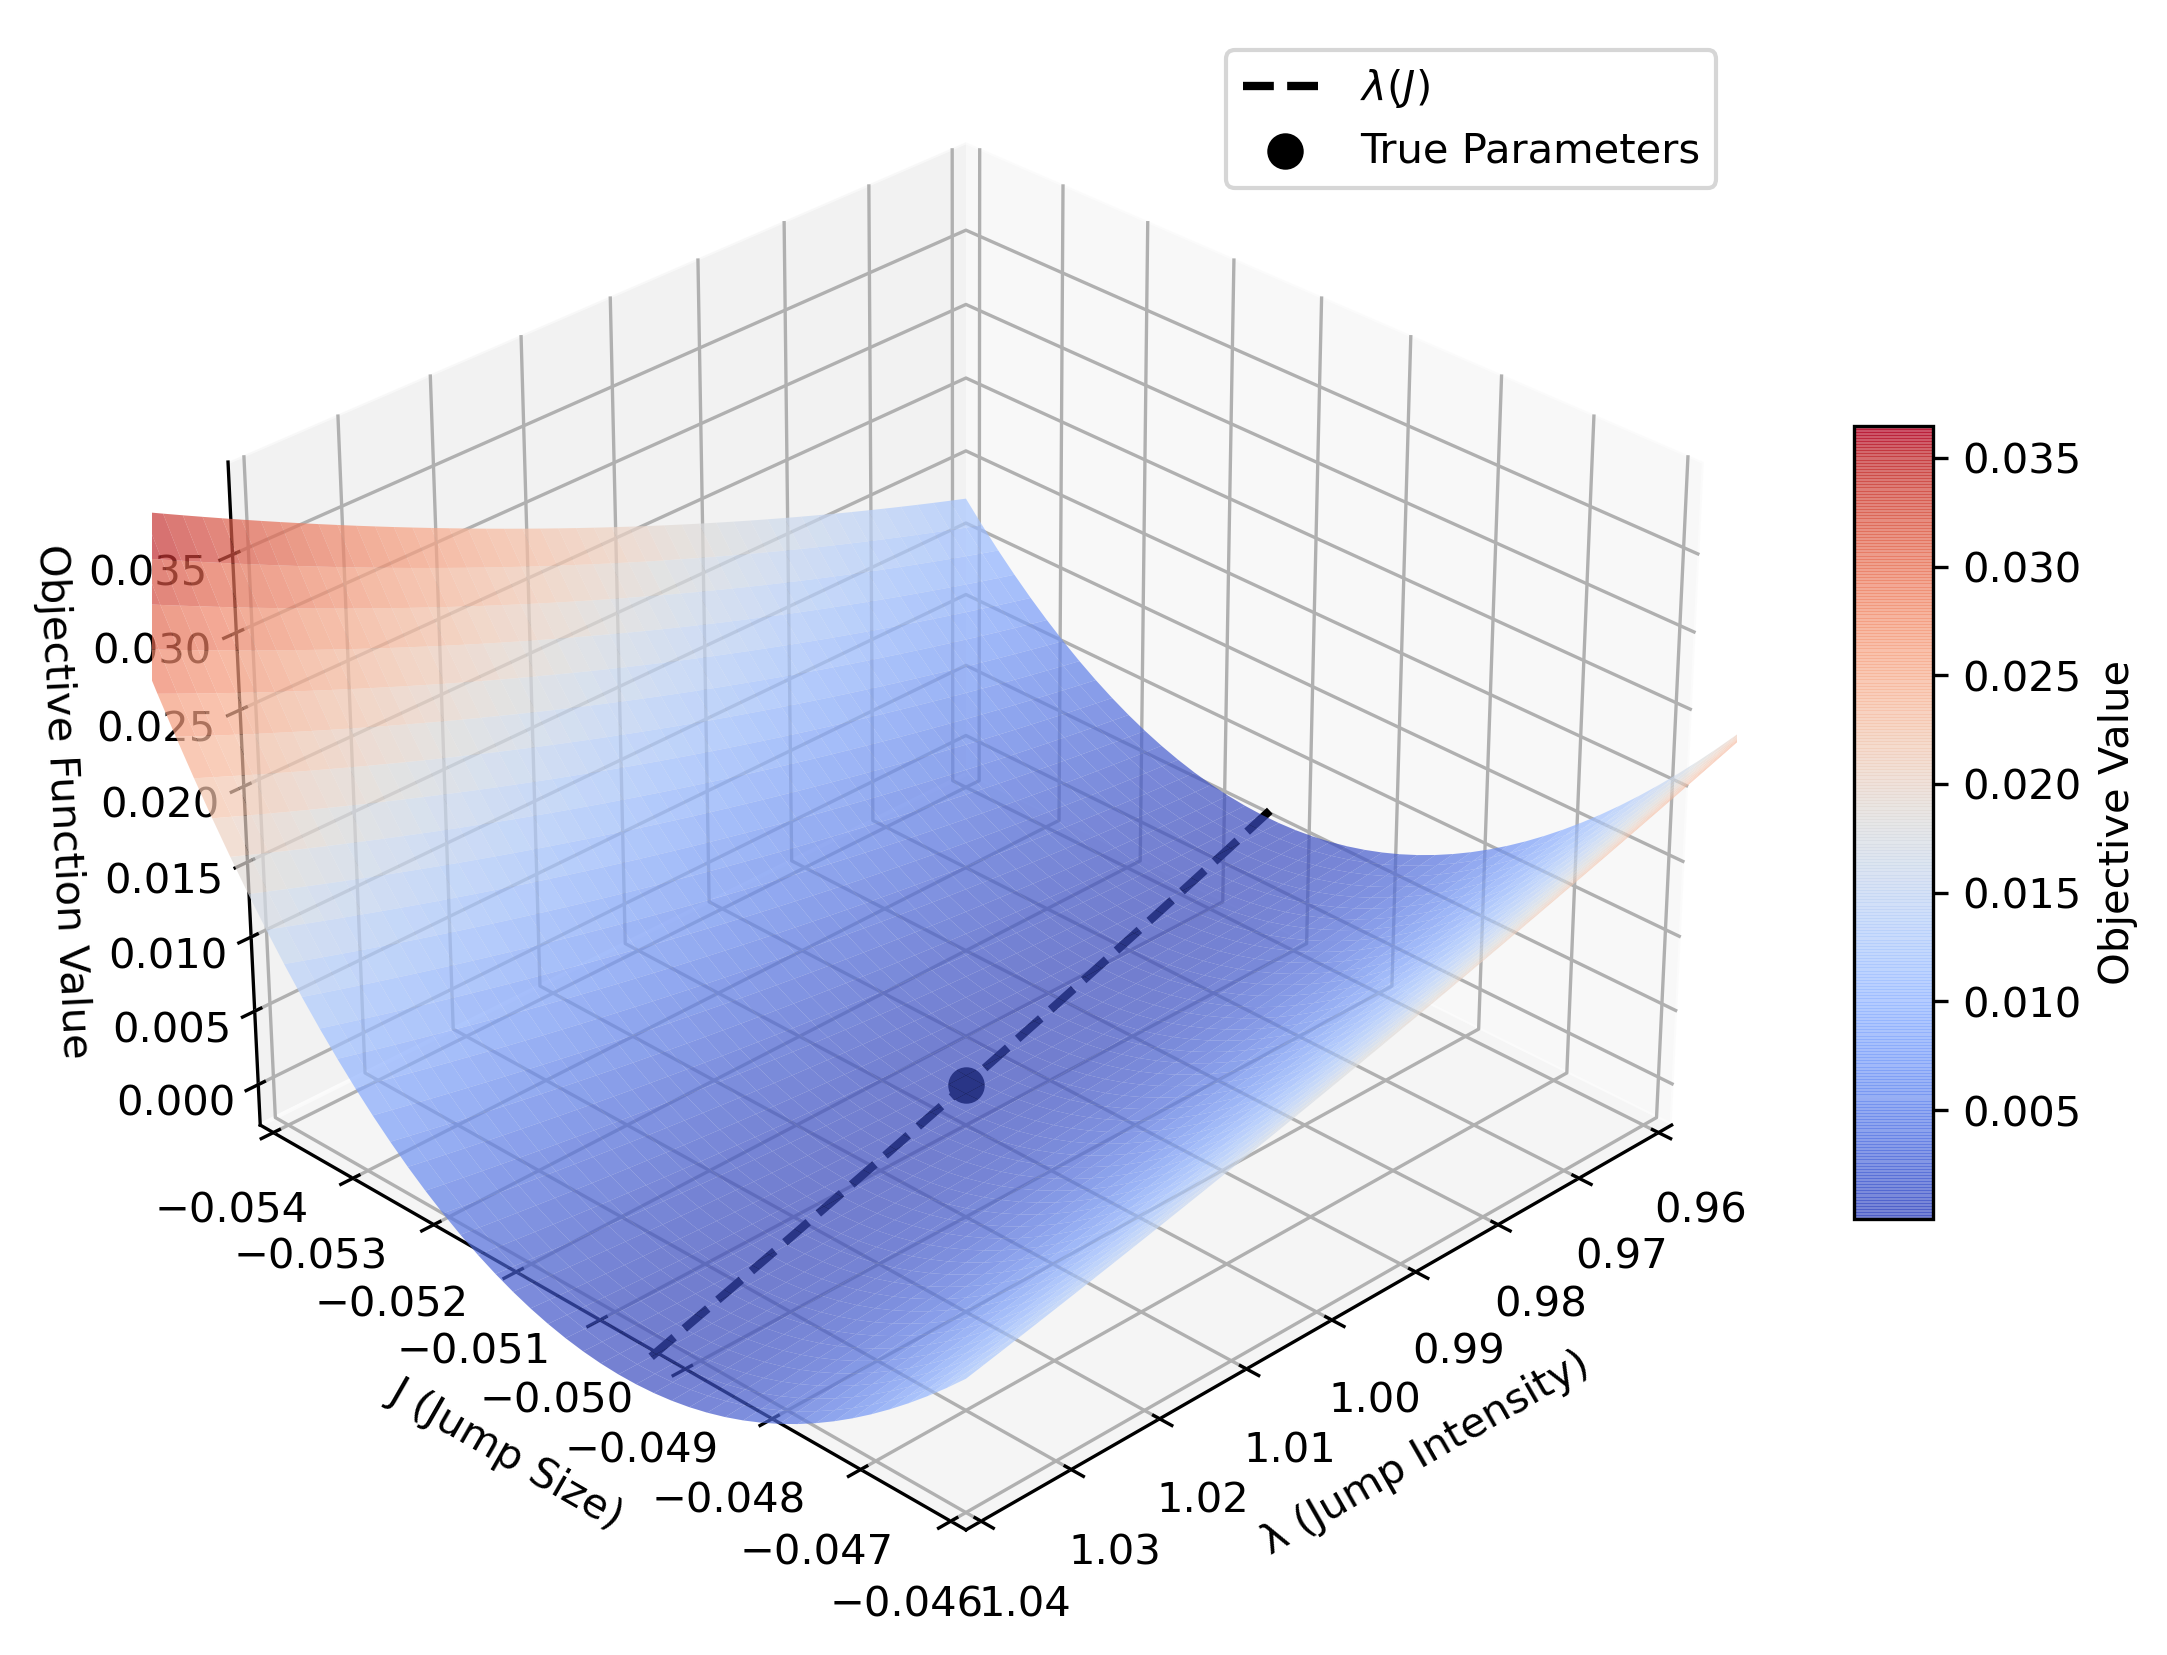
\includegraphics[width=\textwidth]{figs/surface.png} % 
    \end{subfigure}
    \begin{subfigure}{0.48\textwidth}
        \centering
        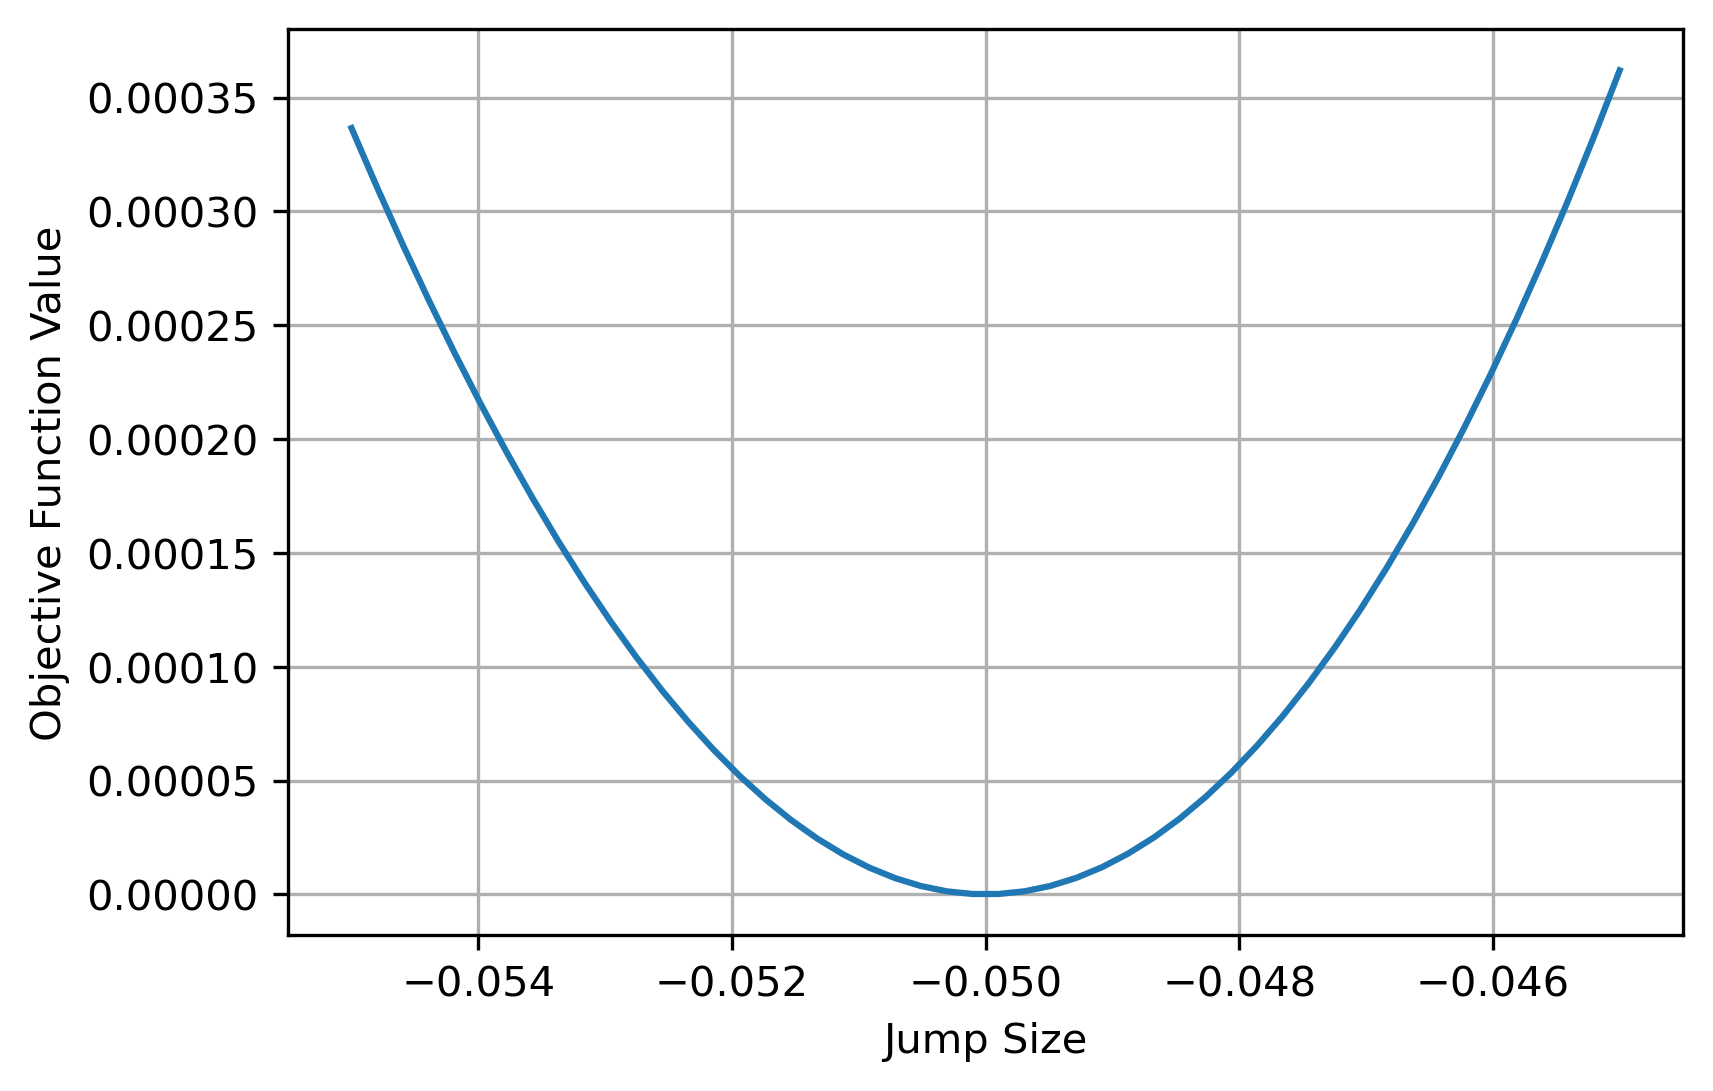
\includegraphics[width=\textwidth]{figs/slice.png} %
    \end{subfigure}
    \caption{Surface (left) of the objective function in \eqref{eq: prop_sjd_21} computed with option prices computed under an SJD process with $\lambda^* = 1, J^* = -0.05$ and $\sigma = 0.16$. Plot of objective function (right/dashed line on left) for parameter values consistent with market observed $VIX$. }
    \label{fig: SJD_sol_locus}
\end{figure}

\begin{proposition}\label{prop: SJD_VIX} 
$S_t$ obeys the SDE in \eqref{eq: SJD} with unknown true parameters $\lambda^*$ and $J^*$ and known diffusive variance $\sigma^2$. If there is a frictionless, arbitrage-free market of European-style options with maturity $T$, then $VIX^2(T; \lambda^*, J^*)$ is identified from option prices and the optimization problem in \eqref{eq: prop_sjd_21} that recovers the unknown parameters can be converted to the univariate problem in \eqref{eq: prop_sjd_22}:
\begin{equation}\label{eq: prop_sjd_21}
  \min\limits_{\lambda, J} \sum\limits_{i=1}^N \left[\sigma^{SJD}(K_i, T; \lambda, J) - \sigma^{mkt}(K_i, T)\right]^2 
\end{equation}
\begin{equation}\label{eq: prop_sjd_22}
  \min\limits_{J}  \sum\limits_{i=1}^N \left[\sigma^{SJD}(K_i, T; \lambda(J), J) - \sigma^{mkt}(K_i, T)\right]^2 
\end{equation}
$\lambda(J)$ in \eqref{eq: prop_sjd_22} is the function:
$$  \dfrac{  VIX^2(T; \lambda^*, J^*)  - \sigma^2 }{2(1+J - e^J)} $$  
Proof provided in appendix.
\qed
\end{proposition}

% This is useful bc... write about how we need only search along the locus of the solution along points consistent with the lambda function
To see how propositions \ref{prop: SJD_VS} and \ref{prop: SJD_VIX} can be useful for calibration, I compute option prices under an SJD models with diffusive variance $\sigma = 0.16$ and jump parameters in a grid centered at $\lambda^* = 1$ and $J^* = -0.05$. The time to maturity $T$ is set to 1/12 (one month). Figure \ref{fig: SJD_sol_locus} plots the values of the objective function in \eqref{eq: prop_sjd_21} for option prices computed under various candidate jump parameters $\lambda$ and $J$ with true parameters $\lambda^* = 1$ and $J^* = -0.05$.\footnote{To compute the error term in equation \eqref{eq: prop_sjd_21}, I sum the squared difference in BSIVs between the prices of OTM options generated under the true parameters and candidate parameters. The strike prices of the OTM options are $ 90, 91, \ldots, 110$ and the spot price is 100.} From the plot we see that, in the neighborhood of the true parameters, the objective function is very flat. As noted by \cite{cont2004nonparametric}, this can be challenging for optimization routines, particularly gradient-based methods, to handle. Since the VIX is observable, we can narrow our parameter search to the locus of points $L$ consistent with the observed level of the VIX:
$$L = \Bigg\lbrace (\lambda, J) \text{ such that }  \lambda =  \dfrac{VIX^{2}(T; \lambda^*, J^*) - \sigma^2}{2(1+J - e^J)} \Bigg\rbrace $$
In the left plot, the dashed line on the surface are the values of the objective function for the set of points in $L$. The right plot displays the values attained by the objective function restricted to just the set of points that lie in $L$. This reduces the problem to searching a flat region of the objective function to a simple univariate line search on $L$. 

\subsubsection{Identification under general processes}\label{subsubsec: theory_general}
Now I consider calibration in the context of a more general price process featuring jumps and stochastic volatility, two salient characteristics represented in modern option pricing models. Suppose the underlying process $S_t$ obeys the following stochastic differential equation (SDE): 
\begin{equation}\label{eq: general_process_sde}
   \dfrac{dS_t}{S_t}=\sqrt{V_t} d W_t+[\exp(J_t) - 1] d N_t- \lambda_t \mu_J d t
\end{equation}
where $\mu_J = \mathbb{E}[\exp(J_t) - 1]$. The above process is quite general, allowing for a separate variance process and general Levy densities for the jump process. $N_t$ is the usual counting jump process with stochastic jump intensity $\lambda_t$. Denote the vector of model parameters for the SDE in \eqref{eq: general_process_sde} by $\Theta$ and define $\mathbb{Q}_\Theta$ to be the pricing measure implied by the process in \eqref{eq: general_process_sde} given $\Theta$. Recycling some notation from before, denote the prices of European-style call and put options with strike $K$ and maturity $\tau$ priced under $\mathbb{Q}_\Theta$ by $C(K,\tau; \Theta)$ and $P(K, \tau; \Theta)$. I assume frictionless markets, the absence of arbitrage, a continuum of observed strike prices, no dividend yield and a risk-free rate of zero. Unlike in the prior section, I assume there are $M$ observed option maturities, $\lbrace\tau_1, \tau_2 \ldots, \tau_M\rbrace$, rather than a single maturity. I consider the inverse problem of recovering the true parameter vector $\Theta^*$ given option prices implied by the SDE in \eqref{eq: general_process_sde}. Like in the prior section, I tackle two cases, one where variance swap prices co-terminal with the option maturities are observed and the other where only the option prices are observed.

Suppose variance swap prices with the same maturities as the options are observed by the econometrician. By no-arbitrage, the variance swap price $VS(\tau; \Theta)$ with maturity $\tau$ under the general model with parameters $\Theta$ is given by:
\begin{equation}\label{eq: general_var_swap}
 VS(\tau;\Theta) = \dfrac{1}{\tau}  \mathbb{E}\left[QV(\tau) \vert \Theta\right] = \dfrac{1}{\tau} \mathbb{E}\left[\int_0^{\tau} V_t  d t + \int_0^{\tau} \int_{\mathbb{R}} J^2 \nu(d s, d x) \Big\vert \Theta\right]
\end{equation}
where $\mathbb{E}(\cdot\vert \Theta)$ is the expectation operator computed using pricing measure $\mathbb{Q}_\Theta$. The variance swaps the econometrician observes in the market, $VS^{mkt}(\tau)$, are priced under the pricing measure associated with the true parameter vector $\Theta^*$, thus  $VS^{mkt}(\tau) =  VS(\tau; \Theta^*)$. 

As before, the econometrician can solve the following optimization problem to recover the parameter $\Theta$:
\begin{equation}\label{eq: general_opt}
    \min\limits_{\Theta} \sum\limits_{j=1}^M\sum\limits_{i=1}^{N_j} w_{i,j} \left[\sigma(K_{i,j}, \tau_j; \Theta) - \sigma^{mkt}(K_{i,j}, \tau_j)\right]^2 
\end{equation}
where $N_j$ is the number of OTM options of maturity $\tau_j$ and $\sigma(K_{i,j}, \tau_j; \Theta)$ denotes the BSIV of an OTM option with strike $K_{i,j}$ and maturity $\tau_j$ priced under the measure $\mathbb{Q}_{\Theta}$. $w_{i,j}$ are non-negative constants which act as weights. $\sigma^{mkt}(K_{i,j}, \tau_j)$ denotes the BSIV of an OTM option priced under the true measure $\mathbb{Q}_{\Theta^*}$, the BSIV observed in the market. Therefore, we have $\sigma^{mkt}(K_{i,j}, \tau_j) = \sigma(K_{i,j}, \tau_j; \Theta^*)$.

To be of practical use, an option pricing model should fit the observed volatility surface well. In addition to this first-order priority, for a variety of research and applied use cases, another desirable property is consistency between this fitted volatility surface and the observed term structure of variance. An obvious application where this property would be important is the hedging variance derivatives (e.g variance swaps, VIX futures) which are often hedged using a portfolio of vanilla options. Other use cases include academic studies which examine variance risk premia through the lens of an option pricing model. To quantify this risk premium in a coherent way, the model-implied level of variance should match what is implied by option prices. To this end, I augment the objective function in \eqref{eq: general_opt} using the regularization terms $g^{VIX}(\Theta)$ and $g^{VS}(\Theta)$ which penalize deviations from the observed term structure of the VIX and variance swap rates respectively:
\begin{equation}\label{eq: reg_term_VIX}
    g^{VIX}(\Theta) = \sum\limits_{j=1}^{M} w^v_j \left[VIX(\tau_j; \Theta) - VIX^{mkt}(\tau_j)\right]^2
\end{equation}
\begin{equation}\label{eq: reg_term_VS}
g^{VS}(\Theta) = \sum\limits_{j=1}^{M} w^v_j \left[\sqrt{VS(\tau_j; \Theta)} - \sqrt{VS^{mkt}(\tau_j)}\right]^2 
\end{equation}
where $w^v_j$ are non-negative constants. The augmented objective function is given in the statement of Proposition \ref{prop: general}. The proposition shows that for the SDE in \eqref{eq: general_process_sde}, $\Theta^*$ minimizes this augmented objective function and that this augmented objective function is observable. 

 \begin{proposition}\label{prop: general} 
 $S_t$ obeys the SDE in \eqref{eq: general_process_sde} with unknown true parameter vector $\Theta^*$. If there is a frictionless, arbitrage-free market of European-style options then $\Theta^*$ solves the minimization problem in \eqref{eq: prop_general_opt} for any non-negative constants $w_{i,j}$ and $w^v_j$:
\begin{equation}\label{eq: prop_general_opt}
\min\limits_{\Theta} \Bigg\lbrace \sum\limits_{j=1}^{M}\sum\limits_{i=1}^{N(\tau_j)} w_{i,j}\left[\sigma(K_i, \tau_j; \Theta) - \sigma^{mkt}(K_i, \tau_j)\right]^2 +  g(\Theta) \Bigg\rbrace 
\end{equation}
where $g(\Theta) = g^{VIX}(\Theta)$. The objective minimized in \eqref{eq: prop_general_opt} is observable solely from option prices. If variance swaps with maturities $\lbrace\tau_j\rbrace_{j=1}^{M}$ are observed, then $g(\Theta) = g^{VS}(\Theta)$ also produces an observable objective function in \eqref{eq: prop_general_opt}. In either case, \eqref{eq: prop_general_opt} is observable even if the stochastic process for $S_t$ is mis-specified. Proof provided in appendix.
\qed
\end{proposition}
Proposition \ref{prop: general} provides an observable objective function in the case where only option prices are observed and where option prices and the variance swap rates are jointly observed. The objective minimized in \eqref{eq: prop_general_opt} is observable even when the SDE in \eqref{eq: general_process_sde} is mis-specified, that is, market prices are generated under a different pricing measure altogether. In the case of model mis-specification, the parameter vector that minimizes the objective is no longer the true parameter vector, but the set of parameters which delivers the model with the closest fit to market option prices and the variance term structure. The fact that the objective function is observable regardless of the correct stochastic process being specified makes it implementable in model calibration. In addition, the functional form, specifically, the non-negative constants $w_{i,j}$ and $w_j^v$, allow for more targeted calibration based on the user's needs. A practitioner needing a tight fit on ATM options could appropriately weight the constants associated with the error in ATM options more heavily. Similarly, a researcher wanting to fit the term structure of the variance swap curve can up-weight the $w_j^v$ constants. The choice of these constants govern the relative importance of certain parts of the volatility surface and variance term structure in model calibration.

One can employ the summations \eqref{eq: reg_term_VIX} and \eqref{eq: reg_term_VS} as informative moment conditions for a generalized method of moments (GMM) framework, reminiscent of the pioneering work of \cite{chernov2000study} and \cite{pan2002jump}. These works incorporate moment conditions under the physical and risk-neutral distributions of the underlying compared to the solely risk-neutral moments used here. The first summation in \eqref{eq: prop_general_opt} can be seen as a moment condition for the implied volatility surface and the second summation as a moment condition for the term structure of variance. The particularly useful case of proposition \ref{prop: general} is the one where only option prices are observed. Typically, assets which have options written on them do not have a corresponding variance swap market.\footnote{Popular equity indices, such as the S\&P 500 or DAX, are notable exceptions as underlyings with actively traded variance swap markets.} Fortunately, while the term structure of the variance swap curve is not observed, one can still recover the $VIX$ term structure which is identical to the variance swap term structure in the case of continuous prices and an approximation in the general case when the underlying can jump.\footnote{The error in this approximation is proportional to the product of the third moment of the jump distribution and the expectation of the jump intensity over the swap's life.} 

Even if the data generating process is not known, the minimization problem is still conceptually valid as a means of obtaining the best fitting parameters. The "best" model obtained in this context is the one that minimizes the objective function. A potential issue is that while the resulting model might match option prices and implied volatilities closely, the model-implied term structure of variance (measured by variance swap prices or the squared VIX) can have substantial error when compared to the term structure observed in the market. Surprisingly, as I show in section \ref{sec: emp_results}, this can be true even for the VIX term structure, quantities directly computed from option prices themselves. In general, fitting the options well in a mean squared error sense does not guarantee fitting the term structure of the VIX or variance swaps well. 

Unfortunately, in nearly all applied contexts, the data generating price process is not known. Indeed, in practice, researchers and practitioners first posit a credible model then calibrate the parameters to minimize some function of model error. Intuitively, a desirable feature for a well-calibrated model is for the quantity below, the error in the calibrated volatility surface, to be small:
$$\sum\limits_{j=1}^{N_\tau}\sum\limits_{i=1}^{N(\tau_j)} \left[\sigma(K_{i,j}, \tau_j; \Theta) - \sigma^{mkt}(K_{i,j}, \tau_j)\right]^2$$ 
Like in a GMM approach to calibration, I minimize a function of the moment conditions rather that require that they hold exactly. Another sensible feature for a well-calibrated model is to fit the term structure of the VIX and/or variance swap quotes furnishing consistency between option and variance swap prices. As in proposition \ref{prop: general}, I can incorporate the term structure of variance or the VIX depending on the observed market instruments. These two considerations motivate a special case of my proposed objective function:
\begin{equation}\label{eq: obj_function_special_case}
    \sum\limits_{j=1}^{M}\sum\limits_{i=1}^{N_{\tau_j}} \left[\sigma(K_{i,j}, \tau_j; \Theta) - \sigma^{mkt}(K_{i,j}, \tau_j)\right]^2 + \sum\limits_{j=1}^{M} N(\tau_j) \left[\sqrt{V(\tau_j; \Theta)} - \sqrt{V^{mkt}(\tau_j})\right]^2
\end{equation}
where $V(\tau_j; \Theta)$ is the model-implied variance swap, when variance swap term structures are observed and is the model-implied VIX term structure otherwise. $V^{mkt}(\cdot)$ denotes the comparable market observed term structure. The first sum in \eqref{eq: obj_function_special_case} is identical to the sums in \eqref{eq: prop_sjd_11} and \eqref{eq: prop_sjd_21}, being simply the sum of squared errors in BSIV space with equal weight on each contract. The second sum is a special case of \eqref{eq: reg_term_VIX} or \eqref{eq: reg_term_VS}, scaling the error in the variance swap or VIX term structure by $N_{\tau_j}$, the number of OTM options of maturity $\tau_j$. This scaling makes errors in fitting $V^{mkt}(\tau_j)$ contribute just as much to the objective function as errors over the entire volatility smile at maturity $\tau_j$. Intuitively, a 1\% error in the variance is "as bad" at maturity $\tau_j$, according to the objective function, as a 1\% error across all contracts with maturity $\tau_j$. Finally, I include a hyperparameter, $\alpha \in [0,1]$, which governs the relative importance between fitting the variance swap/VIX term structure and the option implied volatilities, yielding my proposed objective function below:
\begin{equation}\label{eq: obj_function_general}
 \alpha   \sum\limits_{j=1}^{M}\sum\limits_{i=1}^{N_{\tau_j}} \left[\sigma(K_{i,j}, \tau_j; \Theta^*) +  \sigma^{mkt}(K_{i,j}, \tau_j)\right]^2 + (1-\alpha) \sum\limits_{j=1}^{M} N(\tau_j) \left[V(\tau_j\vert \Theta) - V^{mkt}(\tau_j)\right]^2
\end{equation}
Section \ref{sec: emp_results} is devoted to studying model calibration with the objective function above. I calibrate volatility surfaces using \eqref{eq: obj_function_general} first in a simulation study, then using the SPX volatility surface implied by traded contracts. I also provide guidance for the choice of hyperparameter $\alpha$ which, in empirical settings, can greatly affect quality of calibration. 

One might wonder of what additional benefit can be had by using the information from the variance swap or VIX term structures; after all, the term structure of VIX is itself identified from option prices with the variance swap rate and VIX being highly correlated. However, as I explore further in section \ref{sec: emp_results}, fitting the observed option implied volatilities well does not guarantee a reasonable fit for the VIX term structure when calibrating to market option quotes. In the case the price process is continuous, such in the \cite{heston1993closed} or \cite{heath1992bond} models, the variance swap term structure itself can be subject to the same criticisms as, in the continuous case, this term structure is also identified from option prices. For applied use, I find there are two main benefits from using \eqref{eq: obj_function_general} as the objective function. The first is that introducing an error in term structures regularizes the resulting parameters to match the observed term structure. I find that a simple sum of squared errors objective function, equivalent to $\alpha = 0$ in \eqref{eq: obj_function_general}, produces large errors in both the VIX and variance swap term structures. The introduction of a regularization term based on these term structures, by the appropriate choice of $\alpha > 0$, can produce calibrated models that closely match observed term structures while maintaining a quality fit on the volatility surface.




\section{SPX Option panel and variance term structure}\label{sec: data}
I use the quotes provided by OptionMetrics for European-style call and put options on S\&P 500 Index (SPX). Data coverage begins in January 1996 and ends in August 2023. Quotes are end-of-day 4pm bid and ask prices. For the purposes of calibrating option pricing models, I use the mid-price as the option's price computed from the bid and ask quotes for OTM options. I consider only OTM options for inclusion in the panel as it suffices to price OTM options to be able to price a vanilla option of any strike.\footnote{Since the options are European-style, one can recover the price of in-the-money option from out-of-the-money option prices via a put-call parity relation. From an estimation perspective, OTM options also have the advantage that they generally more liquid compared to the ITM option of the same strike. } Other data include risk-free rates from T-bill rates and dividend yield obtained from Bloomberg. I exclude options from the panel with maturity greater than 1 year.

I impose standard filters on the option data following the literature (e.g. \cite{constantinides2013puzzle},  \cite{goyal2022equity}, etc). These filters eliminate contracts with prices which are either obviously erroneous, violate no-arbitrage conditions, or are so deeply out-of-the-money that their extrinsic value is close to zero. Specifically, I eliminate contracts which have a bid price greater than its ask price, have a ask price less than or equal to 10 cents, imply put-call parity violations, or have a standardized moneyness greater than 6 in absolute value. I compute the standardized moneyness $k_{i,j}$ of an OTM option with time to maturity $\tau_{j}$ and strike price $K_{i,j}$ as:
$$k_{i,j} = \dfrac{\ln\left(K_{i,j}/S_t\right)}{\text{VIX}(\tau_{j})\sqrt{\tau_{j}}}$$
where $\text{VIX}(\tau_{j})$ is the VIX computed using the methodology of \cite{jiang2005model} using options with time to maturity $\tau_{j}$. $S_t$ is the spot price of the index.  After filters are applied, the option panel consists of 2,968,199 call options and 6,182,584 put options.


\begin{table}[!t]
    \centering
\begin{tabular}{lllllll}
\toprule
Moneyness & Maturity & BSIV (\%) & Std. Moneyness & Option price (\%)  & DTE & N Obs. \\
\toprule
\multicolumn{2}{l}{\textit{Panel A: Call options}}  &  &  & &  &    \\ 
ATM & 0-9 DTE & 19.2 & 0.497 & 0.48 & 6.26 & 102,308 \\
 &  & (12.4) & (0.288) & (0.463) & (2.15) &  \\
 OTM & 0-9 DTE & 17.8 & 1.44 & 0.0447 & 6.11 & 82,033 \\
 &  & (10.7) & (0.274) & (0.0511) & (2.19) &  \\
 DOTM & 0-9 DTE & 18.6 & 2.26 & 0.0116 & 5.91 & 10,938 \\
 &  & (12.2) & (0.299) & (0.0111) & (2.27) &  \\
ATM & 10-30 DTE & 16.5 & 0.474 & 0.758 & 20.4 & 461,003 \\
 &  & (8.99) & (0.286) & (0.7) & (5.89) &  \\
OTM & 10-30 DTE & 14.8 & 1.39 & 0.0541 & 19.5 & 247,084 \\
 &  & (7.86) & (0.26) & (0.0601) & (5.99) &  \\
 DOTM & 10-30 DTE & 15.8 & 2.22 & 0.016 & 17.7 & 16,670 \\
 &  & (9.44) & (0.214) & (0.012) & (5.76) &  \\
ATM & 30+ DTE & 16.2 & 0.455 & 1.86 & 130 & 1,549,052 \\
 &  & (6.27) & (0.28) & (1.73) & (90.5) &  \\
OTM & 30+ DTE & 14.7 & 1.32 & 0.134 & 117 & 492,123 \\
 &  & (5.64) & (0.235) & (0.176) & (90) &  \\
DOTM & 30+ DTE & 18.3 & 2.13 & 0.0426 & 115 & 7,988 \\
 &  & (7.56) & (0.123) & (0.0314) & (101) &  \\
 \midrule
\multicolumn{2}{l}{\textit{Panel B: Put options}}  &  &  &  & &      \\
ATM & 0-9 DTE & 22.7 & -0.499 & 0.602 & 6.26 & 102,728 \\
 &  & (14.3) & (0.289) & (0.481) & (2.15) &  \\
  OTM & 0-9 DTE & 25.6 & -1.49 & 0.156 & 6.23 & 97,635 \\
 &  & (14.6) & (0.288) & (0.119) & (2.16) &  \\
 DOTM & 0-9 DTE & 29.6 & -3.24 & 0.0357 & 6.23 & 184,172 \\
 &  & (13.3) & (0.891) & (0.0267) & (2.16) &  \\
ATM & 10-30 DTE & 21.1 & -0.489 & 1.02 & 20.6 & 495,907 \\
 &  & (10.4) & (0.287) & (0.68) & (5.87) &  \\
 OTM & 10-30 DTE & 24.4 & -1.48 & 0.295 & 20.2 & 393,474 \\
 &  & (10.8) & (0.288) & (0.168) & (5.94) &  \\
 DOTM & 10-30 DTE & 29.2 & -3.18 & 0.0739 & 19.7 & 620,642 \\
 &  & (10.3) & (0.841) & (0.0458) & (6.01) &  \\
ATM & 30+ DTE & 22.7 & -0.489 & 2.55 & 134 & 1,759,255 \\
 &  & (7.59) & (0.287) & (1.58) & (90.8) &  \\
OTM & 30+ DTE & 28.1 & -1.46 & 0.716 & 129 & 1,315,187 \\
 &  & (8.73) & (0.287) & (0.386) & (91.2) &  \\
DOTM & 30+ DTE & 32.2 & -2.81 & 0.17 & 98.4 & 1,213,584 \\
 &  & (9.22) & (0.619) & (0.0971) & (76.2) &  \\
\bottomrule
\end{tabular}
    \caption{Summary statistics of S\&P 500 Index option panel. BSIV and option prices (normalized by index spot price) are expressed as percentages. The N Obs. (number of observations) column reports the number of option contracts observed in each category.  }
    \label{tab:summary_stats}
\end{table}

Table \ref{tab:summary_stats} presents summary statistics of the option panel, separated into call and put options. These contracts are further divided by their standardized moneyness and maturity. An option $i$ is in the ATM (at-the-money), OTM (out-of-the-money), or DOTM (deep OTM) bucket if the absolute value of its standardized moneyness $\vert k_{i,t} \vert$ is in $[0,1), [1,2), \text{ or } [2,\infty)$ respectively. Options are sorted into different maturity categories based on the number of days to expiration (DTE): 1-9 DTE, 10-30 DTE, or 30+ (31-365) DTE. For both put and call options, I pick up the presence of a volatility smile. On average, the ATM options possess the lowest BSIV while the DOTM are the highest within their respective maturity categories for both puts and calls. This is most pronounced for put options with DOTM options having the highest BSIVs across both panels reflecting the relatively high cost of hedging large negative jumps \citep{bollerslev2011tails}.

The largest categories of options are the 30+ DTE categories consisting mostly of standard expiration index options.\footnote{Standard expiration options are AM-settled and expire on the third Friday of each month. } The shorter maturities, which mostly consist of non-standard weekly expirations, are less represented in the full sample, despite their contemporary popularity. Across all maturity categories, we observe a volatility skew: OTM put options have greater BSIV on average than OTM call options of similar maturity. This skew in implied volatility units is largest at maturities greater than 30 days. For these maturities, an average OTM put option is nearly twice as expensive as the average OTM call option in implied volatility terms. These observations are consistent with empirical work documenting the properties of volatility surfaces generated by index options \citep{gatheral2011volatility}.

\begin{figure}[!t]
    \centering
    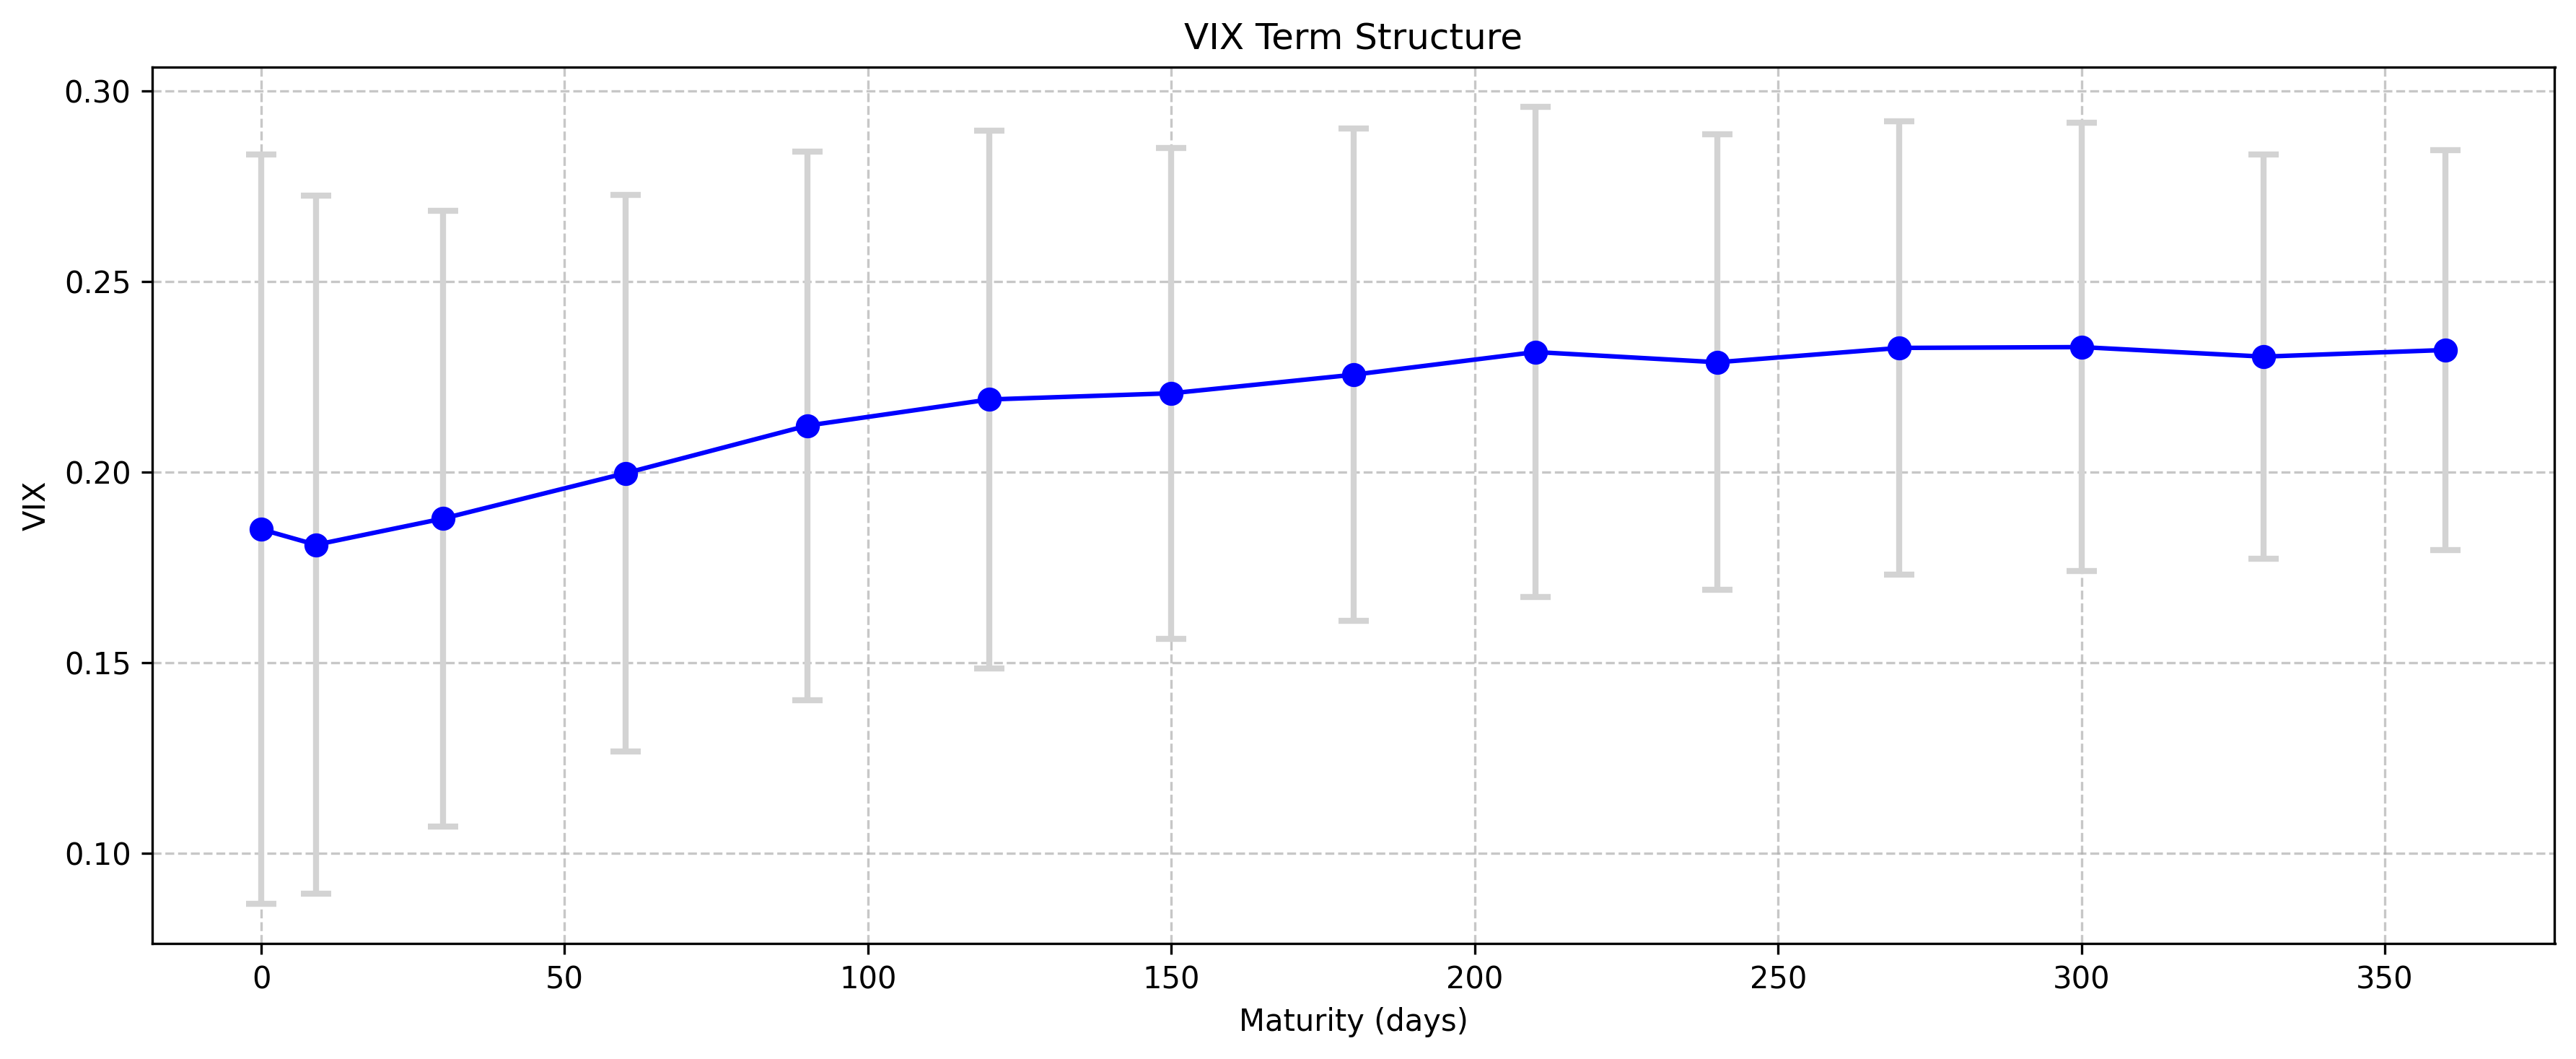
\includegraphics[width=1\linewidth]{figs/VIX_avg_term_structure.png}
    \caption{Mean (blue dots) with standard error bars of the VIX at the 9 day and 1 to 12 month horizon computed from option prices of the appropriate maturity. }
    \label{fig:VIX_term_strct}
\end{figure}

Turning to the term structure of variance, I compute the VIX Index at a number of horizons using the VIX formula in \eqref{eq: disc}. To get a sense of a typical term structure for the SPX, I calculate VIX across several horizons and compute its unconditional mean and standard deviation for each horizon. I compute the VIX for each monthly horizon between 1 and 12 months using the closest option maturity to the given horizon. I also replicate CBOE's 9-day VIX, choosing the closest option maturity between 8 and 10 days as the inputs for the VIX formula.\footnote{CBOE interpolates the VIX on days when the exact target maturity is not listed using nearby maturities. The resulting quantities are nearly identical to the ones I compute here. } I plot the mean and standard deviation of these VIX indices in figure \ref{fig:VIX_term_strct}. 

Consistent with observations made by prior studies (e.g. \cite{dew2017price}, \cite{johnson2017risk}), the term structure of the VIX is typically upward-sloping, flattening out around the intermediate horizons. The error bars around the unconditional averages shows substantial variability in the VIX at all horizons, with the short end of the term structure exhibiting higher volatility as compared to the long end. 


\section{Empirical results}\label{sec: emp_results}
In this section, I apply my calibration framework to two contexts: a simulation study and a calibration exercise on SPX options. To work with a model sufficiently complex for the calibration to be challenging, I consider the calibration of the \cite{bates1996jumps} model in both setups. The Bates model combines the stochastic volatility process of \cite{heston1993closed} with the jump process from \cite{merton1976option}, effectively nesting both models. In section \ref{subsec: simulations}, I demonstrate the ability of the framework to recover model parameters given the option prices generated under the Bates model. In section \ref{subsec: SPX_fit}, I calibrate a Bates model to the SPX equity index options panel constructed in section \ref{sec: data}. Lastly, in section \ref{subsec: SPX_jump_process}, I show how the calibrated parameters can shed light on the role of jumps in the overall price fluctuations of the S\&P 500.

Before proceeding with my empirical exercises, I define Bates model here and provide some useful closed-form expressions for the VIX and variance swap term structure. Denote underlying's price by $S_t$ and the latent variance process by $V_t$. $S_{t-}$ denotes the price level at time $t$ prior to a jump. I suppress time subscripts whenever an expression's meaning is unambiguous. The Bates model assigns these processes the following dynamics:
\begin{equation}
\begin{aligned}
& d S_{t-}=\left(r-q-\lambda \mu_J\right) S_{t-} d t+\sqrt{V_t} S_{-t} d W_t+(e^{J_t}-1) S_{t-} d N_t \\
& d V_t=\kappa\left(\theta-V_t\right) d t+\sigma_V \sqrt{V_t} d W_t^v \\
& \mathbb{E}\left[d W_t  d W_t^v\right]= \rho d t \\
& \mathbb{P}\left(d N_t=1\right)=\lambda d t\\
& J_t \sim Normal\left(\log \left(1+\mu_J\right)-\frac{\sigma_J^2}{2}, \sigma_J^2 \right)
\end{aligned}
\end{equation}
For the Bates model, the parameter vector is $\Theta = [V_t, \kappa, \theta, \sigma_v, \rho, \lambda, \mu_J, \sigma_J]$. $V_t$ is the latent level of variance, driven by a Brownian motion with variance proportional to its own level, $\sigma_V^2 V_t$, and is a mean-reverting process with long term variance $\theta$ and speed of adjustment $\kappa$. $\rho$ is the instantaneous correlation between the two Brownian motions. The jump process $J_t$ is drawn from a Gaussian distribution with mean $\log(1+\mu_J) - \sigma^2_J/2$ and variance $\sigma_J^2$ and has arrival intensity $\lambda$. On arrival, the underlying price instantly changes by $S_{t-}[\exp(J_t) - 1]$.

\cite{broadie2008effect} derive the variance swap term structure in closed form for the Bates model, allowing for straight-forward computation as a function of the model parameters. The variance swap rate $VS(\tau; \Theta)$ implied by the model is given by:
\begin{equation}\label{eq: var_swap_bates}
VS(\tau; \Theta) =\theta+\frac{V_0-\theta}{\kappa \tau}\left(1-e^{-\kappa \tau}\right) + \lambda \left[(\log(1+\mu_J) - \sigma^2_J/2)^2 + \sigma_J^2\right]
\end{equation}
Combining \eqref{eq: var_swap_bates} with equation \eqref{eq: VIX_gap} allows us to compute a closed form expression for the squared VIX term structure:
$$VIX^2(\tau; \Theta) = VS(\tau\vert \Theta) - 2\lambda\mathbb{E}(1 + J + J^2/2 - e^J\vert \Theta)$$ 
where expectation $\mathbb{E}(\cdot\vert \Theta)$ is taken over the risk-neutral distribution under the Bates model with parameter vector $\Theta$. Computing the relevant moments of the jump distribution and $\mathbb{E}(e^J)$, we have: 
$$\mathbb{E}(e^J) = \exp(\log(1 + \mu_J)-\sigma^2_J/2 + \sigma^2_J/2) = 1+\mu_J$$
$$\mathbb{E}(J) = \log(1 + \mu_J)-\sigma^2_J/2 $$
$$\mathbb{E}(J^2) = \left[\log(1 + \mu_J) - \sigma^2_J/2\right]^2 + \sigma^2_J$$
Substituting moments and simplifying, I derive a closed-form formula for the $VIX$ term structure implied by the Bates model: 
\begin{equation}\label{eq: bates_VIX}
VIX^2(\tau; \Theta)  = VS(\tau; \Theta) - 2\lambda\left(\log(1+\mu_J) - \mu_J + \frac{1}{2}[\log(1+\mu_J) - \sigma_J^2/2]^2\right)
\end{equation}

For the purposes of pricing options in the Bates model, I use the PROJ method of \cite{kirkby2015efficient}, a Fourier-based pricing method that employs series truncation, allowing for computationally efficient computation of option prices.\footnote{For obtaining option prices under the Bates model, I use the python implementation of the PROJ method from the fyfy library. The Github repository can be found here: \href{https://github.com/jkirkby3/fypy}{fypy Github repo}.}

  \begin{table}[!t]
    \centering
\begin{tabular}{lllllllll}
\toprule
 Parameter:  & $V_0$ & $\kappa$ & $\theta$ & $\sigma_v$ & $\rho$  & $\lambda$ & $\mu_J$ & $\sigma_J$ \\
\midrule
 Initial value $(\Theta_0)$  & 0.0576 & 2.03 & 0.04 & 0.38 & -0.7  & 0.59 & -0.05 & 0.07 \\
\hline Uniform distribution lower bound (a) & 0.01 &  0.01 & 1 & 0.1 &  -1 &  0 & -0.1 & 0.0\\
 Uniform distribution upper bound (b) & 0.1 & 0.1 & 5 & 0.5 & 1 & 5 & 0.1 & 0.1 \\
 \bottomrule
\end{tabular}
    \caption{Initial parameters $\Theta_0$ used by \cite{lindstrom2008sequential} in their simulation study of the Bates model. Parameters are based on the analysis by \cite{bakshi1997empirical} of calibrated Bates models fitted to S\&P 500 Index options. Lower and upper bounds of uniform noise in equation \eqref{eq: simulations}. }
    \label{tab:init_params}
\end{table}


\subsection{Simulation study}\label{subsec: simulations}
As a proof of concept, I simulate option prices from the Bates model, using a broad range of parameter values and attempt to recover the model parameters. Specifically, I first form a set $\mathcal{P}$ of parameter vectors as follows. Table \ref{tab:init_params} displays the parameter values from a simulation study on the Bates model conducted by \cite{lindstrom2008sequential}. I stack these parameters into the vector $\Theta_0$. I generate 1,000 parameter vectors in $\mathcal{P}$ by adding uniformly distributed random variables pointwise to $\Theta_0$, where the lower and upper bound of the uniform distribution for each parameter:
\begin{equation}\label{eq: simulations}
    \Theta_i = \Theta_0 +  
\begin{pmatrix}
Uniform[a_v, b_v] \\
Uniform[a_\kappa, b_\kappa] \\
Uniform[a_\theta, b_\theta] \\
Uniform[a_\sigma^v, b_\sigma^v] \\
Uniform[a_\rho, b_\rho] \\
Uniform[a_\lambda, b_\lambda] \\
Uniform[a_\mu, b_\mu] \\
Uniform[a_\sigma^J, b_\sigma^J] \\ 
\end{pmatrix} \quad\quad \text{ for } i \in \lbrace 1, \ldots, 1000\rbrace
\end{equation}


The bounds of the uniform distribution were chosen to obtain a diverse range of model parameters and to exclude the possibility non-nonsensical parameters being drawn, such as drawing a value greater than 1 for the correlation parameter $\rho$. For each of the 1,000 parameter vectors in $\mathcal{P}$, I calibrate the model using the objective function in \eqref{eq: obj_function_special_case} using $\Theta_0$ as the initial guess for the optimization routine.  To explore the effect of the hyperparameter $\alpha$ on calibration, I show estimation results for a grid of values for $\alpha \in [0,1]$. Table \ref{tab:simulation_results} summarizes the results from this calibration exercise. 

Each of the 1,000 parameter vectors in $\mathcal{P}$, corresponds to a simulated volatility surface. For each run of the simulation, the spot price of the underlying is 100 and its dividend yield is 3\%. The risk-free rate is set to 2\%. I compute option prices under the model for the 1 week (7 days), 1 month (30 days), 3 month (91 days), 6 month (182 days) and 1 year (365 days) maturities with strike prices ranging from 75 to 125, spaced apart by \$1. For the calibration step, I use only OTM options with price greater than or equal to 10 cents. I minimize objective function in \eqref{eq: obj_function_special_case}, using the simulated volatility surface and the VIX for each available maturity using the relation derived earlier in equation \eqref{eq: bates_VIX}. 

\begin{table}[!t]
    \centering
\begin{tabular}{lrrrrrrr}
\toprule
$\text{Hyperparameter } (\alpha):$ & 0.00 & 0.10 & 0.25 & 0.50 & 0.75 & 0.90 & 1.00 \\
\midrule
\multicolumn{8}{l}{\textit{Panel A - Average errors in model-implied BSIVs with VIX}}\\
$\text{Contract Moneyness: }$ &   &   &   &   &   &   &   \\
ATM $(0 \leq \vert k_{i,t}\vert < 1)$  & 2.05\% & 0.12\% & 0.13\% & 0.13\% & 0.14\% & 0.15\% & 0.16\% \\
OTM $(1 \leq \vert k_{i,t}\vert < 2)$ & 3.77\% & 0.21\% & 0.23\% & 0.25\% & 0.26\% & 0.26\% & 0.28\% \\
DOTM $(2 \leq \vert k_{i,t}\vert)$ & 7.74\% & 0.35\% & 0.37\% & 0.41\% & 0.41\% & 0.42\% & 0.44\% \\
\midrule
\multicolumn{8}{l}{\textit{Panel B - Average errors in model-implied BSIVs with variance swap approximation}}\\
$\text{Contract Moneyness: }$ &   &   &   &   &   &   &   \\
ATM $(0 \leq \vert k_{i,t}\vert < 1)$ & 1.98\% & 0.19\% & 0.19\% & 0.17\% & 0.17\% & 0.16\% & 0.16\% \\
OTM  $(1 \leq \vert k_{i,t}\vert < 2)$ & 3.75\% & 0.28\% & 0.29\% & 0.29\% & 0.28\% & 0.27\% & 0.28\% \\
DOTM $(2 \leq \vert k_{i,t}\vert)$  & 7.78\% & 0.45\% & 0.44\% & 0.45\% & 0.45\% & 0.42\% & 0.44\% \\
\midrule 
\multicolumn{8}{l}{\textit{Panel C - Proportion of simulations where parameter vector was exactly recovered}}\\
$\text{Calibration type: }$ &   &   &   &   &   &   &   \\
Exact VIX & 0\% & 56.8\% & 56.6\% & 55.9\% & 56.3\% & 55.7\% & 55.4\% \\
Approximated VIX & 0\%  & 1.4\%  & 1.5\%  & 1.5\%  & 2.2\%  & 3.3\% & 55.4\%\\
\bottomrule
\end{tabular}
    \caption{Average errors for simulated contract prices across for different buckets of standardized moneyness (Panel A and B). Errors broken down by the absolute value of standardized moneyness $\vert k_{i,t} \vert$. Range given in parentheses. Percentage of simulations where parameter vector was exactly recovered (Panel C). }
    \label{tab:simulation_results}
\end{table}


Panel A of table \ref{tab:simulation_results}  records the average error in terms of BSIVs across simulations for models calibrated using different values of the hyperparameter $\alpha$, broken down by different levels of standardized moneyness. Higher values of $\alpha$ correspond to objective functions placing greater weight on the option BSIV surface. At the lower extreme, $\alpha = 0$ corresponds to the case where only information from the VIX term structure is used to calibrate the surface. The errors are much higher compared to average errors under other values of $\alpha$. At the other end, a value of $\alpha = 1$, corresponds to the case where only information from the option BSIVs are used in calibration. The average errors in this case are substantially lower than those under the $\alpha = 0$ case. Figure \ref{fig: VIX_fits} show the average model error of the 1 month and 1 year VIX across the 1,000 simulations in percentages. All values of $\alpha$ produce small errors with the fit becoming perfect as $\alpha \to 0$. For $\alpha = 0.5$, which places equal weight on the VIX term structure and the volatility surface, the error is around 10 basis points for both the 1 month and 1 year VIX. The errors in the VIX term structure are comparable to what we see in the volatility surface fits. Overall, intermediate values of $\alpha$ show similarly low errors suggesting the viability of using an objective function which jointly considers the fit in volatility surface and the variance term structure. These observations suggest a fairly benign trade-off between fitting the volatility surface and VIX term structure at higher values in the unit interval.
 
As discussed in section \ref{sec: theory}, the VIX is based on the pricing formula of a variance swap under the assumption that the underlying price process is continuous. In the presence of jumps, the VIX formula does not necessarily recover the variance swap price, which under no-arbitrage is the risk-neutral expectation of the quadratic variation. However, a number of studies do not make this distinction, treating the square of the VIX as the expected risk-neutral variance or, equivalently under no-arbitrage, as the fair strike of a variance swap.\footnote{\cite{martin2017expected} points out that the VIX, rather than measuring variance, is more accurately categorized as a measure of statistical entropy. \cite{bondarenko2014variance} documents the discrepancy between the VIX construction and the payoff of traded variance swaps. } As pointed out by \cite{carr2012variance} and \cite{ait2020term}, the gap between the squared VIX and the expected quadratic variation is time-varying and at times can be substantial. Despite this, the VIX is widely used as a measure of expected volatility. I consider calibration in this commonly mis-specified case where the VIX is used as an approximation for the variance swap rate. I again calibrate models across different values of $\alpha$; this time using the option BSIV surface and the variance swap curve as inputs for the objective function in \eqref{eq: obj_function_special_case}. Specifically, the variance term structure errors in my objective function are replaced by the following approximation: 
\begin{equation}\label{eq: vix_gap_2}
    \sum\limits_j \left[\sqrt{VS(\tau_j; \Theta)} - \sqrt{VS^{mkt}(\tau_j)} \right]^2 \approx  \sum\limits_j \left[\sqrt{VIX^2(\tau_j; \Theta)} - \sqrt{VS^{mkt}(\tau_j)} \right]^2 
\end{equation}

\begin{figure}[!t]
    \centering
    % First subfigure
    \begin{subfigure}{0.495\textwidth}
        \centering
        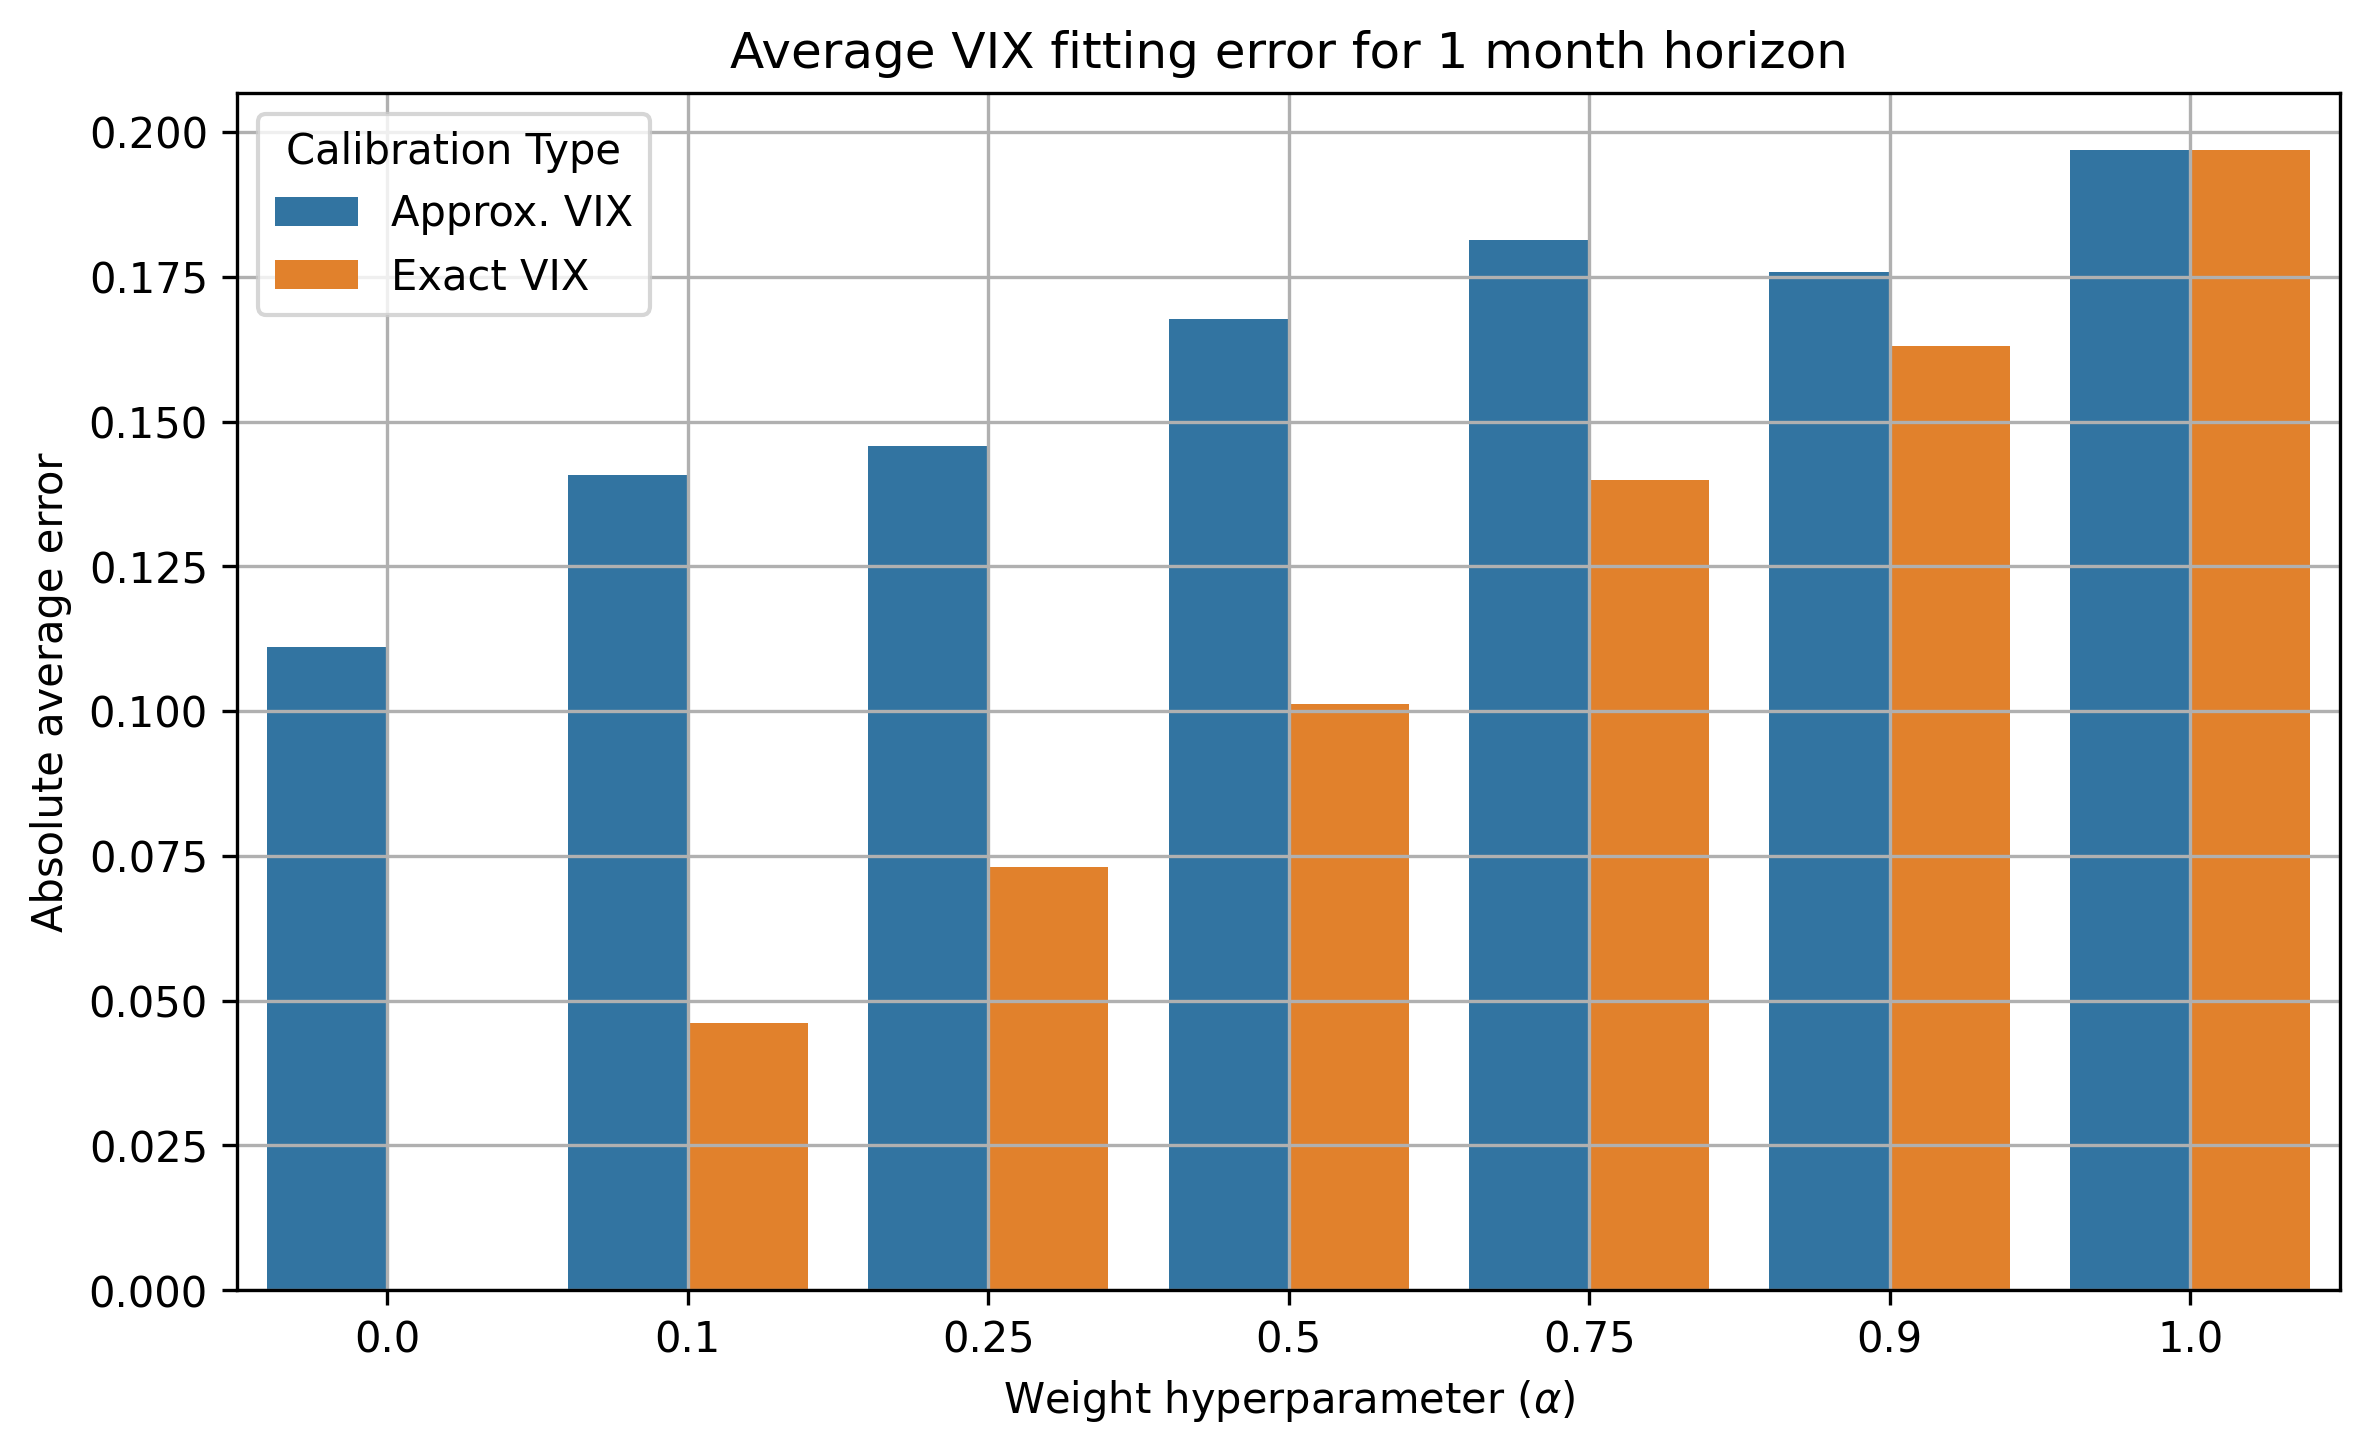
\includegraphics[width=\textwidth]{figs/VIX_fitting_error_30.png} %
    \end{subfigure}
    % Second subfigure
    \begin{subfigure}{0.495\textwidth}
        \centering
        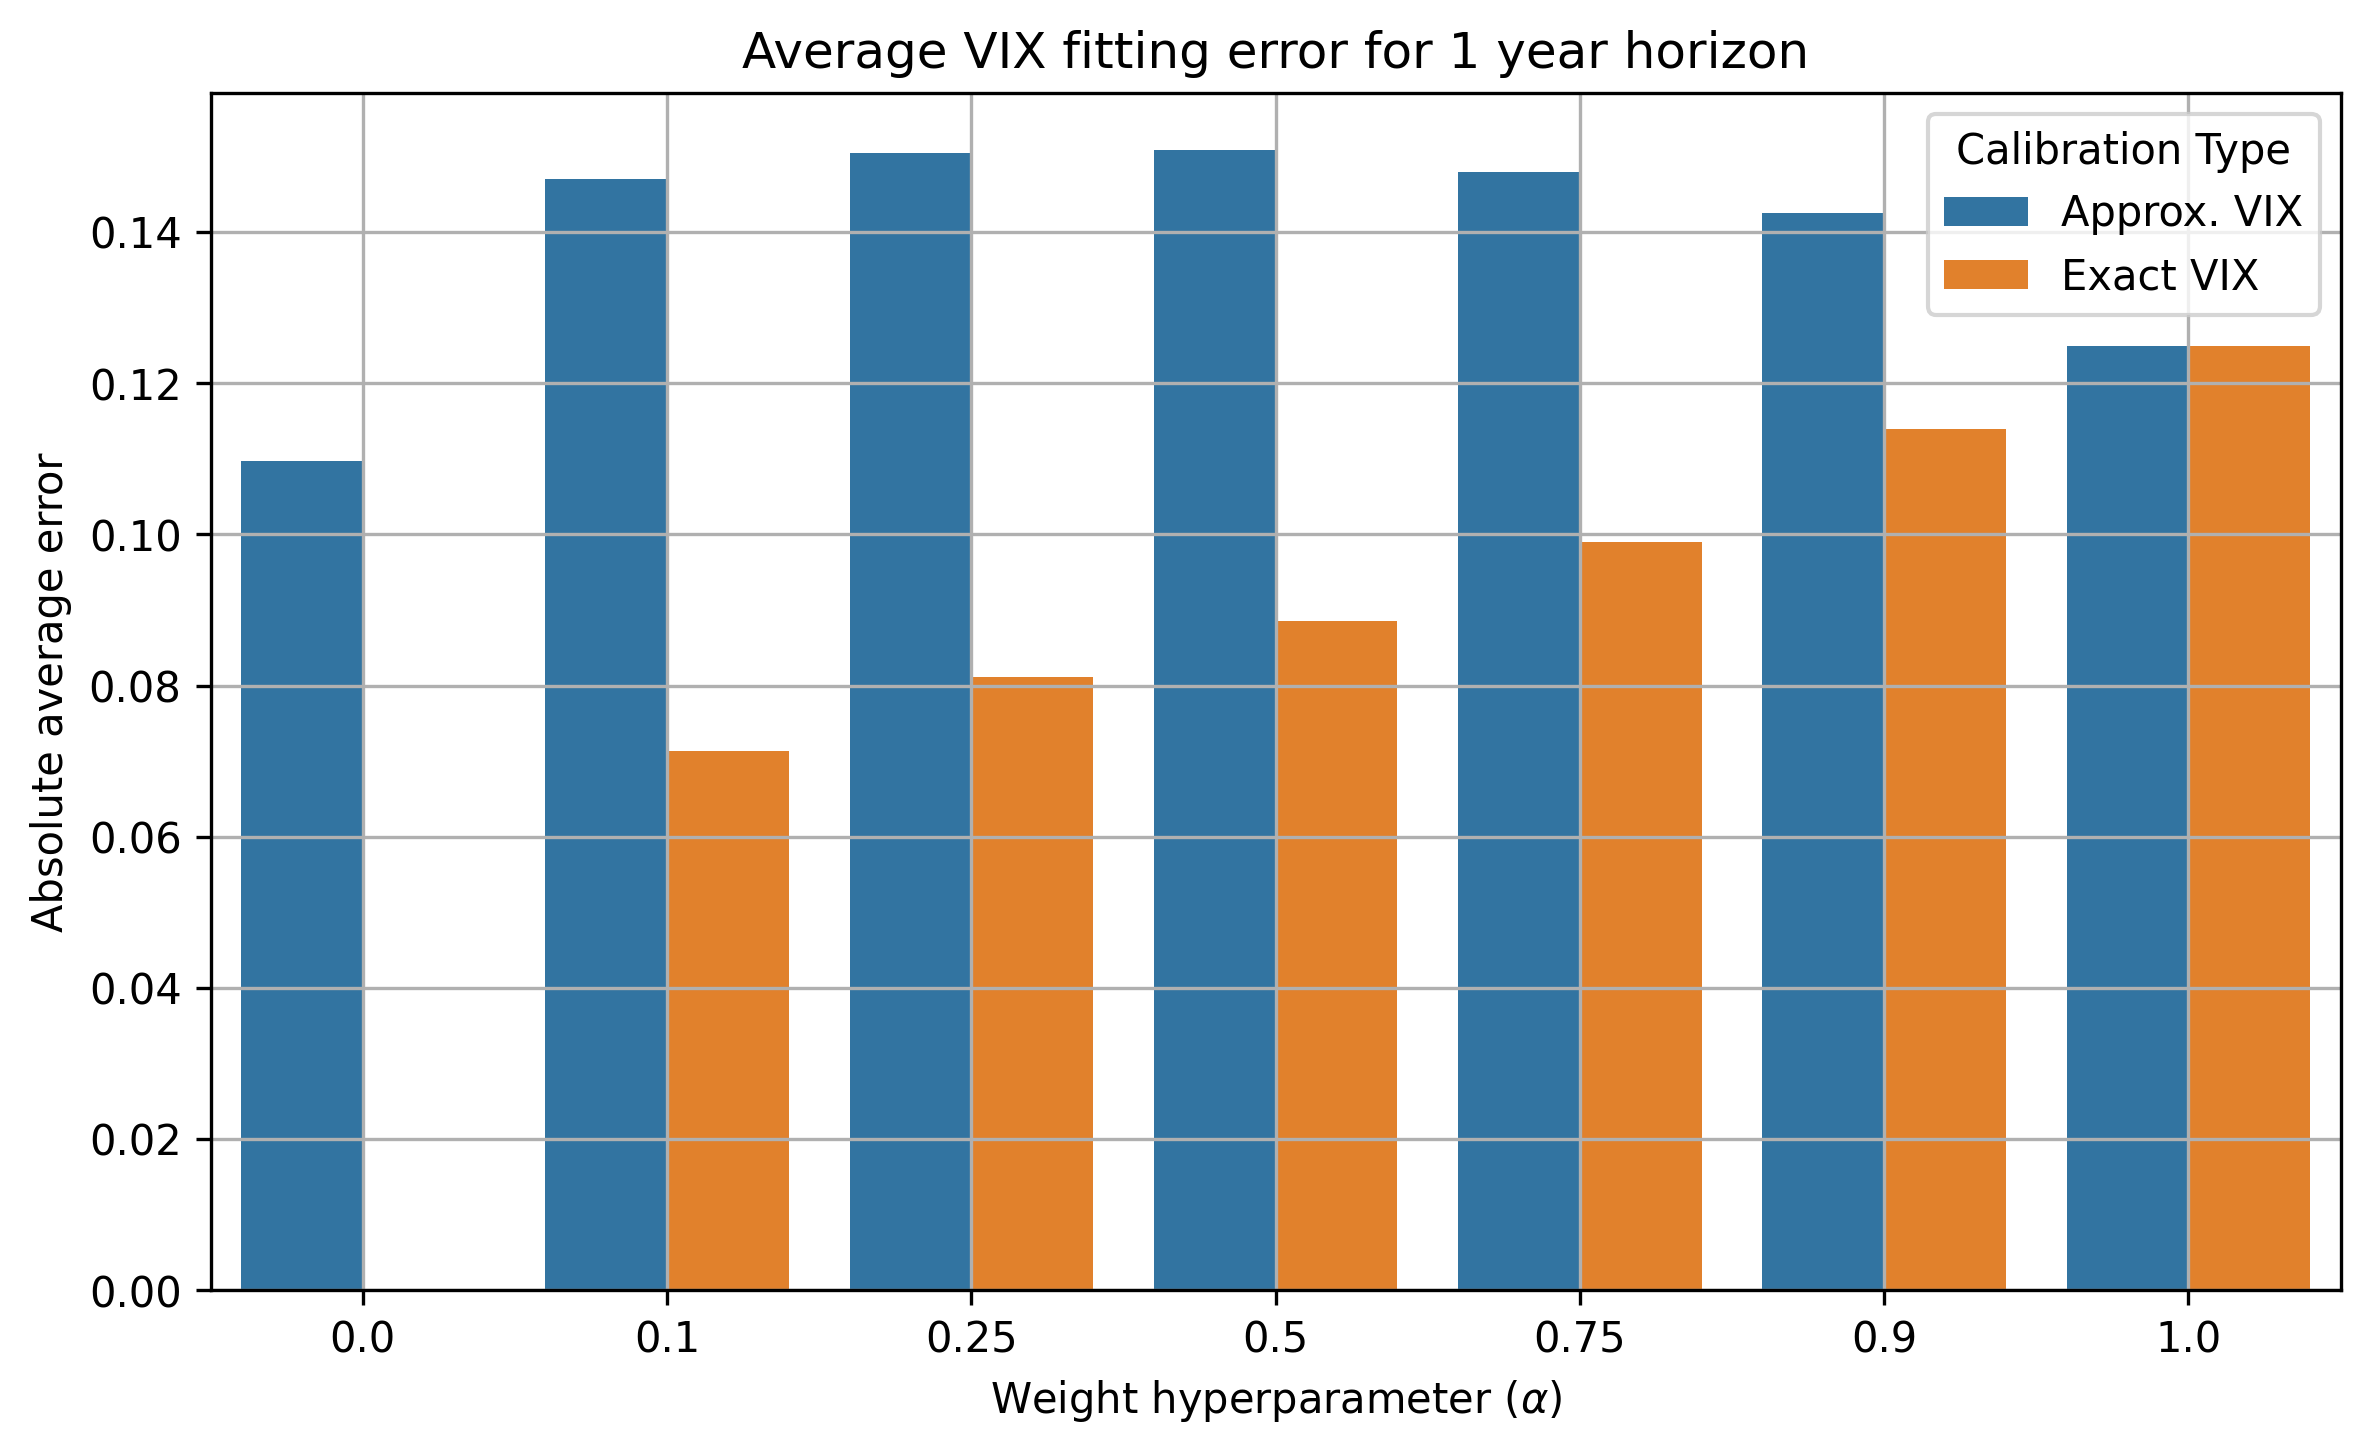
\includegraphics[width=\textwidth]{figs/VIX_fitting_error_365.png} % 
    \end{subfigure}
    
    \caption{Average fitting error (expressed as a percentage) for the 1 month and 12 month VIX over 1,000 simulations. Orange bars show fitting errors for calibration using the exact VIX term structure. Blue bars show fitting errors when using the VIX as an approximation of the variance swap rate.}
    \label{fig: VIX_fits}
\end{figure}

Panel B of table \ref{tab:simulation_results} displays the results from using the common VIX-variance swap expected quadratic variation approximation. For many moneyness categories, the errors are higher when calibrating using the variance swap approximation compared to using the VIX term structure exactly. Although the errors are not substantially higher, the real difference is observed in panel C. Panel C reports the percentage of the 1,000 simulations which recovered the exact true parameters across a range of hyperparameter values. When $\alpha = 0$, we see that under either calibration the exact parameters are never recovered. This is due to the flexibility of the Bates model, as there are multiple parameter vectors consistent with the variance term structure generated in each simulation. From the remaining values of $\alpha$, two salient details stand out; first, using the approximated term structure is substantially worse when it comes to exact recovery of the model parameters. This exercise suggests caution should be applied when using the squared VIX as the expected quadratic variation when it comes to model calibration. Using the exact VIX term structure recovers the parameters more than half of the time exactly and when the exact parameters are not recovered the fitting error across the term structure and volatility surface is low. Second, when using the exact VIX term structure for calibration as in panel A instead of using VIX as an approximation the exact parameters are recovered at nearly identical rates $(\approx 56\%)$ across different values of $\alpha$, excluding the case where $\alpha = 0$. This provides further evidence that the trade-off in goodness-of-fit between the variance term structures and the volatility surface is mild for intermediate values of $\alpha$. 



\subsection{Model calibration to SPX Index options}\label{subsec: SPX_fit}
In this section, I calibrate the Bates model to the SPX Index options data for each day of observations in my option panel using the objective function in \eqref{eq: obj_function_special_case}. The data starts in January of 1996 and ends in August of 2023. To get a sense of the effect the hyperparameter $\alpha$ has on calibration, I calibrate the Bates model for each of the values of $\alpha$: 0, 0.1, 0.25, 0.5, 0.75, 0.9, 1.0. To assess the model fit across the volatility surface and VIX term structure, I compute the average absolute fitting error across different groupings of maturities in table \ref{tab:mae_iv} for call options, put options, and the VIX term structure. The averages are taken over all fitted option prices and values computed from the VIX formula in \eqref{eq: disc} across all trading days in the panel.

Examining the panels of table \ref{tab:mae_iv} by maturity grouping, we see that the most challenging components of the VIX term structure and the volatility surface are located at the shortest maturities. The errors for call and put options with 1 - 9 days to maturity have the highest errors in implied volatility space relative to other maturities. The calibration results on the SPX equity index options are most directly comparable with \cite{broadie2007model} study of S\&P 500 futures options data ranging from 1987 to 2003. The authors estimate the \cite{bates1996jumps} model using options between 10 and 180 days to expiration and obtain authors report an average error of 0.6\% in BSIV terms. I obtain similar results for comparable maturities in my panel for call and put options with 10-30 DTE and 30+ DTE. This is notable even in light of the fact the volatility surfaces in my panel are more challenging from an calibration perspective due to the proliferation of short maturity, weekly expirations which the models need to fit jointly with longer maturities. These very short maturity options have populated contemporary volatility surfaces with many more near-term maturities which been known to be difficult to fit \citep{bandi2024local, bandi0dte}. 

Turning to the short maturity options (1-9 DTE), I observe unsurprisingly higher errors relative to longer maturities. The shortest maturity segment of the volatility surface is notoriously difficult to fit. \cite{andersen2017short} studies options with less than 10 days to maturity and finds that many parametric option pricing models use jump processes at odds with the thickness and time-variation of the jump tails. Using a Bates model-like approach they obtain an average error of 1.24\% on models fitted on only their short maturity sample. The results here are comparable despite having to fit the entire surface out to the 1 year maturity. For values of $\alpha > 0$, the errors for the (1-9 DTE) category are all between $1.47\%$ and $1.58\%$ for call options and $1.53\%$ to $1.67\%$  for put options.

\begin{table}[!t]
\begin{tabular}{lrrrrrrr}
\toprule
Hyperparameter ($\alpha$) & 0.0 & 0.1 & 0.25 & 0.5 & 0.75 & 0.9 & 1.0 \\
\midrule
\textit{Panel A: Calls} &  &  &  &  &  &  &  \\
Call (1--9 DTE) & 4.21\% & 1.58\% & 1.56\% & 1.52\% & 1.49\% & 1.47\% & 1.48\% \\
Call (10--30 DTE) & 4.65\% & 0.68\% & 0.66\% & 0.62\% & 0.59\% & 0.57\% & 0.57\% \\
Call (30+ DTE) & 6.13\% & 1.04\% & 0.96\% & 0.88\% & 0.83\% & 0.79\% & 0.74\% \\
\midrule
\textit{Panel B: Puts} &  &  &  &  &  &  &  \\
Put (1--9 DTE) & 5.57\% & 1.67\% & 1.62\% & 1.58\% & 1.55\% & 1.54\% & 1.53\% \\
Put (10--30 DTE) & 5.06\% & 0.82\% & 0.75\% & 0.71\% & 0.67\% & 0.66\% & 0.65\% \\
Put (30+ DTE) & 5.06\% & 0.75\% & 0.72\% & 0.68\% & 0.65\% & 0.62\% & 0.58\% \\
\midrule 
\textit{Panel C: VIX term structure} &  &  &  &  &  &  &  \\
1--9 DTE & 1.17\% & 1.18\% & 1.21\% & 1.27\% & 1.37\% & 1.53\% & 3.98\% \\
10--30 DTE & 0.45\% & 0.46\% & 0.47\% & 0.51\% & 0.60\% & 0.77\% & 3.14\% \\
30+ DTE & 0.30\% & 0.31\% & 0.32\% & 0.36\% & 0.42\% & 0.50\% & 1.85\% \\
\bottomrule
\end{tabular}
\caption{Mean absolute errors of in model implied volatilities for OTM options (panel A and B) and VIX term structure (panel C) across maturities. Maturities/option maturities used in replication given in round parentheses. }
\label{tab:mae_iv}
\end{table}

Panel C of table \ref{tab:mae_iv}, presents the mean absolute fitting errors for the VIX term structure. As expected, the lowest average error for all maturities occurs at $\alpha = 0$. When $\alpha$ is zero, the entire error in contract implied volatilities drops out of the objective function, leaving only information from the term structure to guide calibration. Indeed, without the error in contract BSIVs term, the fit in the implied volatility surface is sharply poorer for every maturity relative to all other values of $\alpha$. In contrast, a value of $\alpha = 1$ results in the poorest fit to the VIX term structure. Despite poor fit in option BSIVs and therefore prices, the objective function with $\alpha = 0$ delivers a quality fit for the VIX term structure. This illustrates a familiar phenomenon with flexible option pricing models such as the Bates model and is consistent with we was observed with the simulations in section \ref{subsec: simulations}: there are a number of pricing measures that can produce nearly identical variance term structures. At the other extreme, $\alpha = 1$ represents an important special case since it is equivalent to the conventional mean squared error objective used in a wide range of academic and industry applications.  As noted above, the volatility surface fits when $\alpha = 1$ are comparable to literature standards; however, average errors in the model-implied VIX term structures are the highest across the grid of $\alpha$ hyperparameters examined here. Relative to historical averages, the model-implied VIX term structures have average percentage errors across maturities range from between 10\% to 20\% of their average levels. As we calibrate the objective function with values of $\alpha$ less than to 1, the calibrated models imply VIX term structures with substantially smaller errors. For example, in the 10-30 DTE category, the average error of models calibrated with $\alpha = 0.9$ is reduced by $75\%$ compared to models calibrated with $\alpha = 1$. 

\begin{figure}[!t]
    \centering
    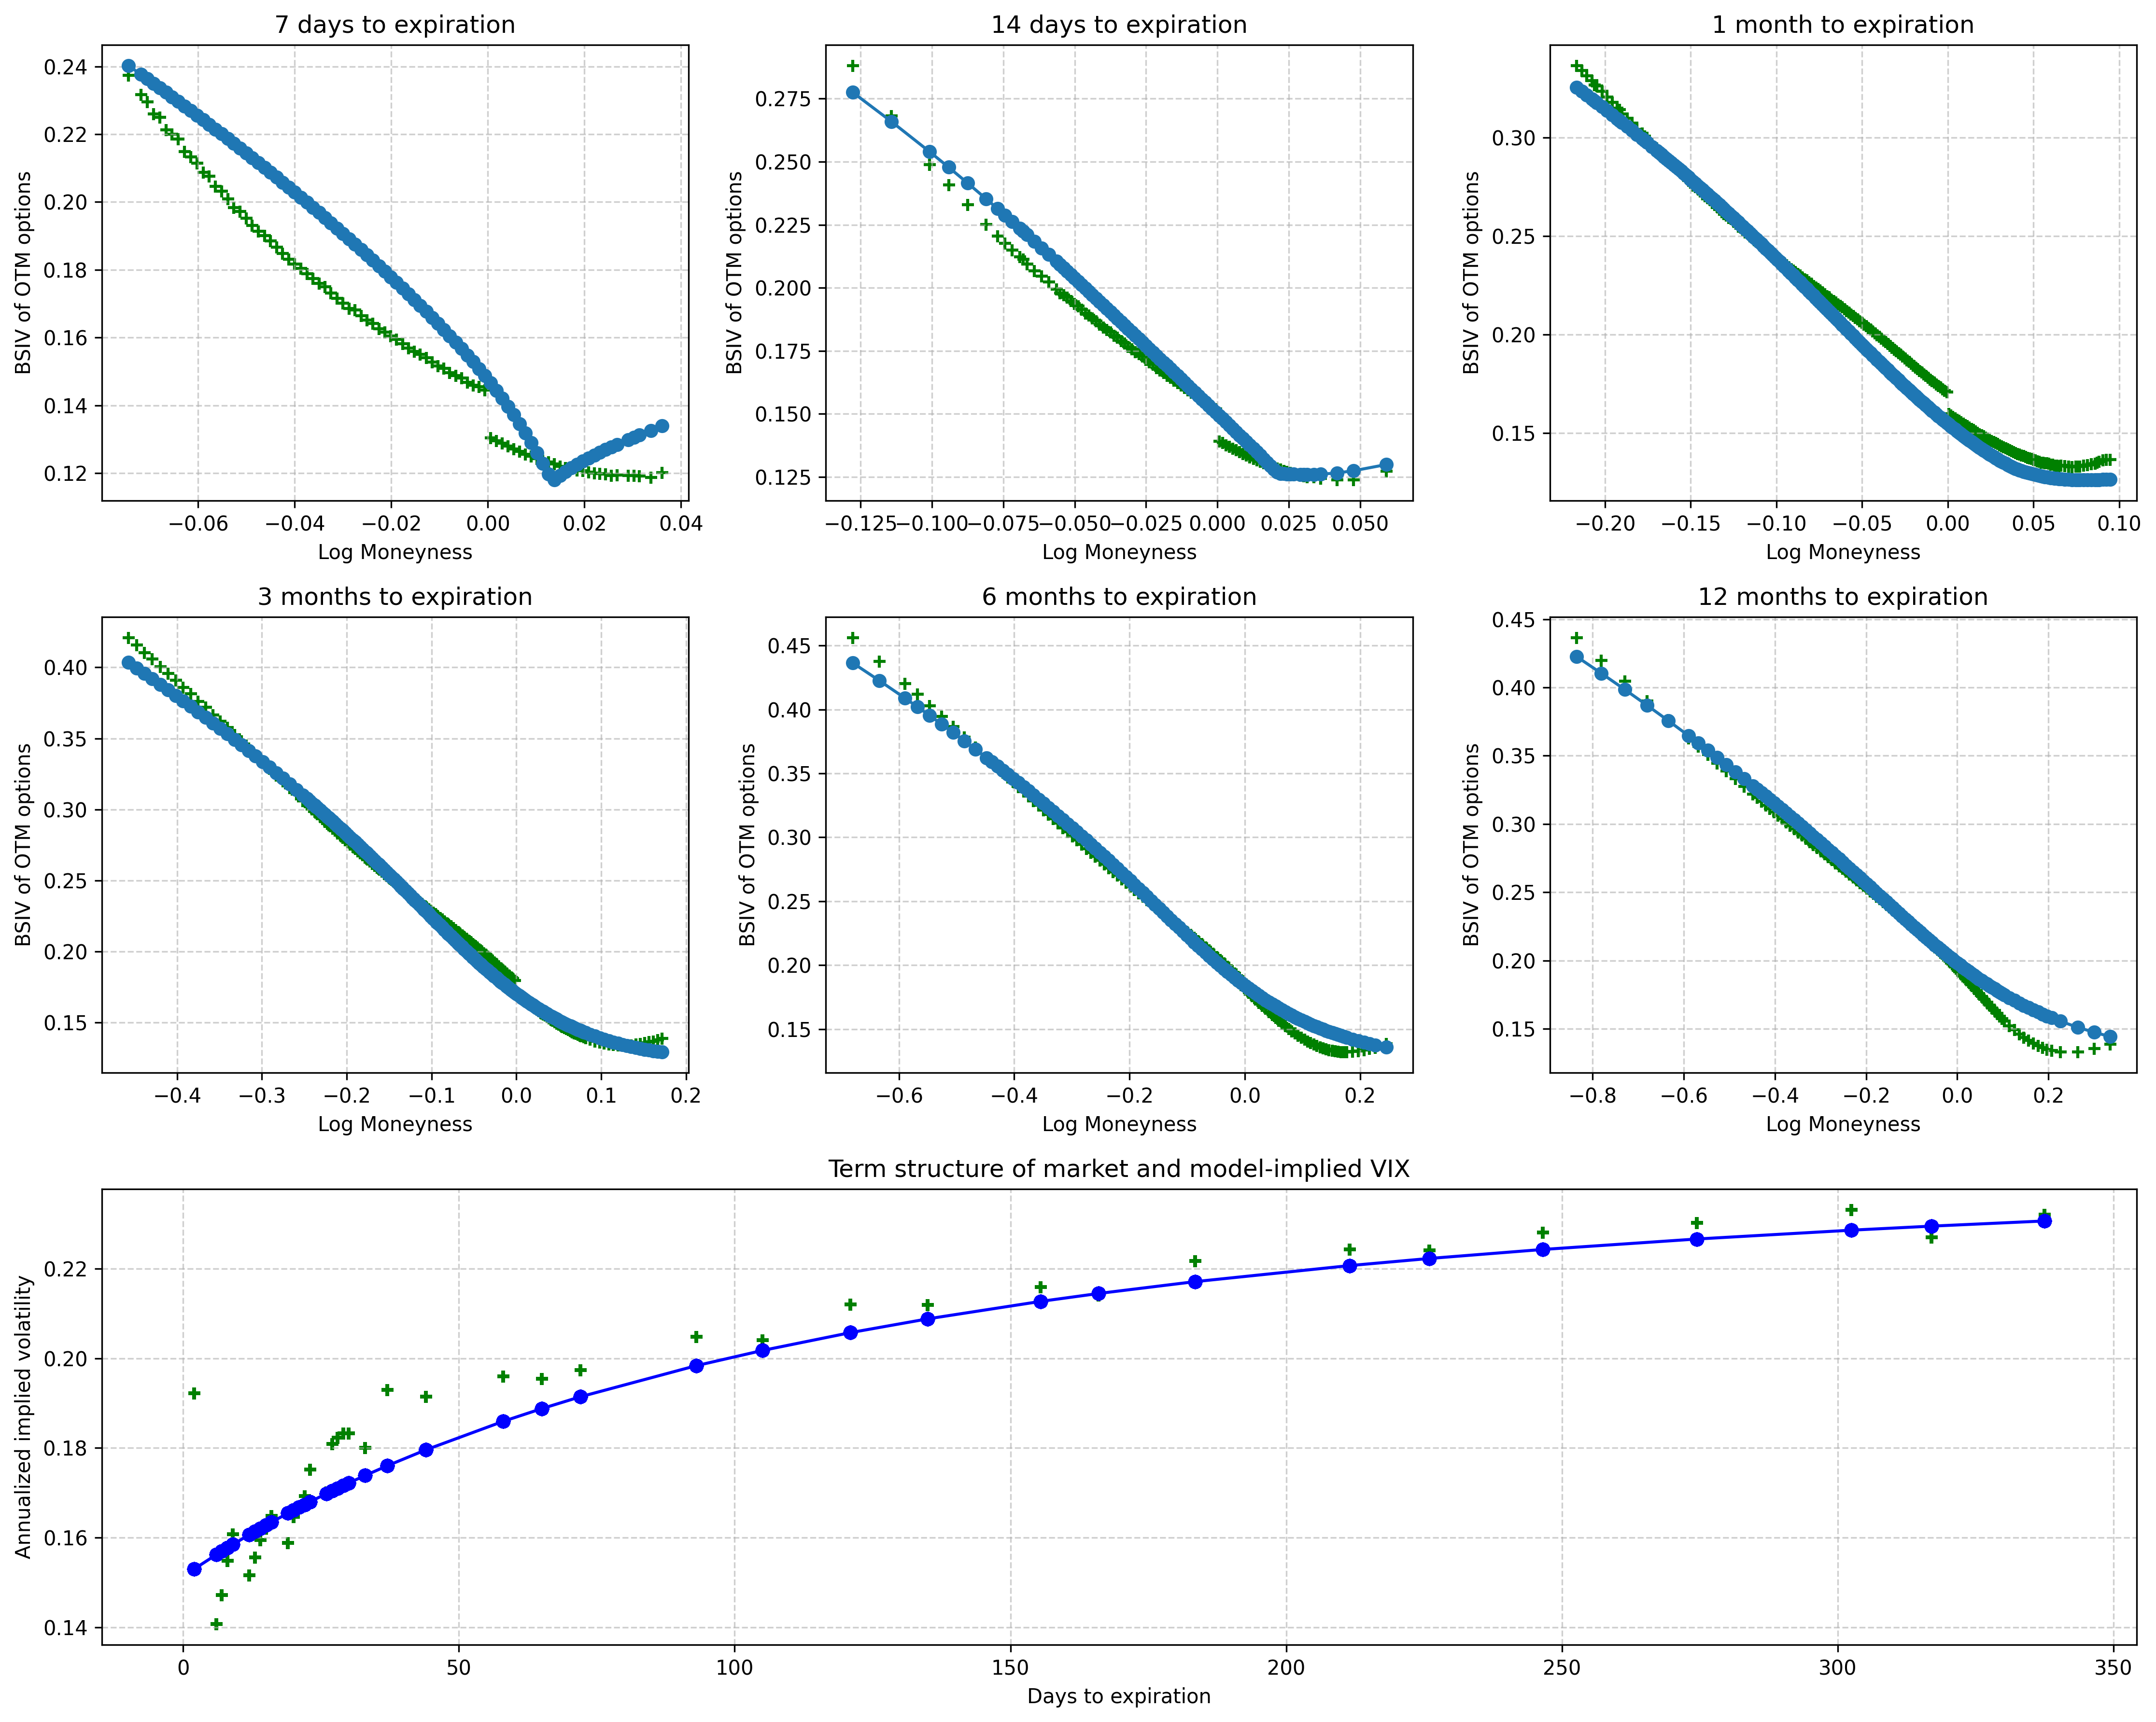
\includegraphics[width=0.9\linewidth]{figs/iv_and_var_swaps.png}
    \caption{Fitted volatility smiles for OTM options on 15th of February 2023. 1 week, 2 week, 1 month, 3 month, 6 month and 12 month maturities plotted in top and middle panels. Fitted and observed VIX term structure plotted on the bottom panel. Fitted quantities are in blue and observed market implied volatilities and options market-implied VIX in green.  }
    \label{fig:model_fits}
\end{figure}

Figure \ref{fig:model_fits} shows the fit of the Bates model on February 15, 2023, a day with a typical level of spot and implied volatilities using the objective function in \eqref{eq: obj_function_general} with $\alpha = 0.9$. The figure plots the fitted implied volatility smiles for select maturities in panel for that day: 7 days, 14 days, 1 month, 3 months, 6 months, and 12 months to maturity. The model-implied smiles for OTM options are plotted in blue and the corresponding market implied volatility smiles are plotted in green. The 7 day model-implied smile highlights some of the weaknesses of the Bates model, namely the inability to fit the steeper volatility smiles observed in very shortest maturities. For intermediate and longer term options, the implied volatility smile fits are reasonable. In the bottom panel, I plot the model-implied VIX (blue curve) and option market-implied VIX (green points). 

Overall, the results from this numerical exercise suggest a relatively high value of $\alpha$ is best for jointly calibrating the volatility surface and the term structure of the VIX. I find minimal trade-offs between fitting the observed VIX term structure and the volatility surface when calibrating the model with values of $\alpha$ close to 1. Table \ref{tab:simulation_results} shows that choosing a value of $\alpha$ close to but strictly less than 1, can calibrate complex option pricing models that simultaneously produce a quality fit to the variance term structure and option volatility surface jointly. Combining the results on the SPX panel with the results from the simulation exercise suggests a value of $\alpha = 0.75$ or $\alpha = 0.9$ for applied use. This is quantitatively similar to a conclusion arrived at by \cite{andersen2015parametric} who use an objective function that uses a regularization term penalizing deviations from spot variance and place a similarly low weight on their variance penalty term and most of the weight on errors in contract-level BSIVs. 

\begin{figure}
    \centering
    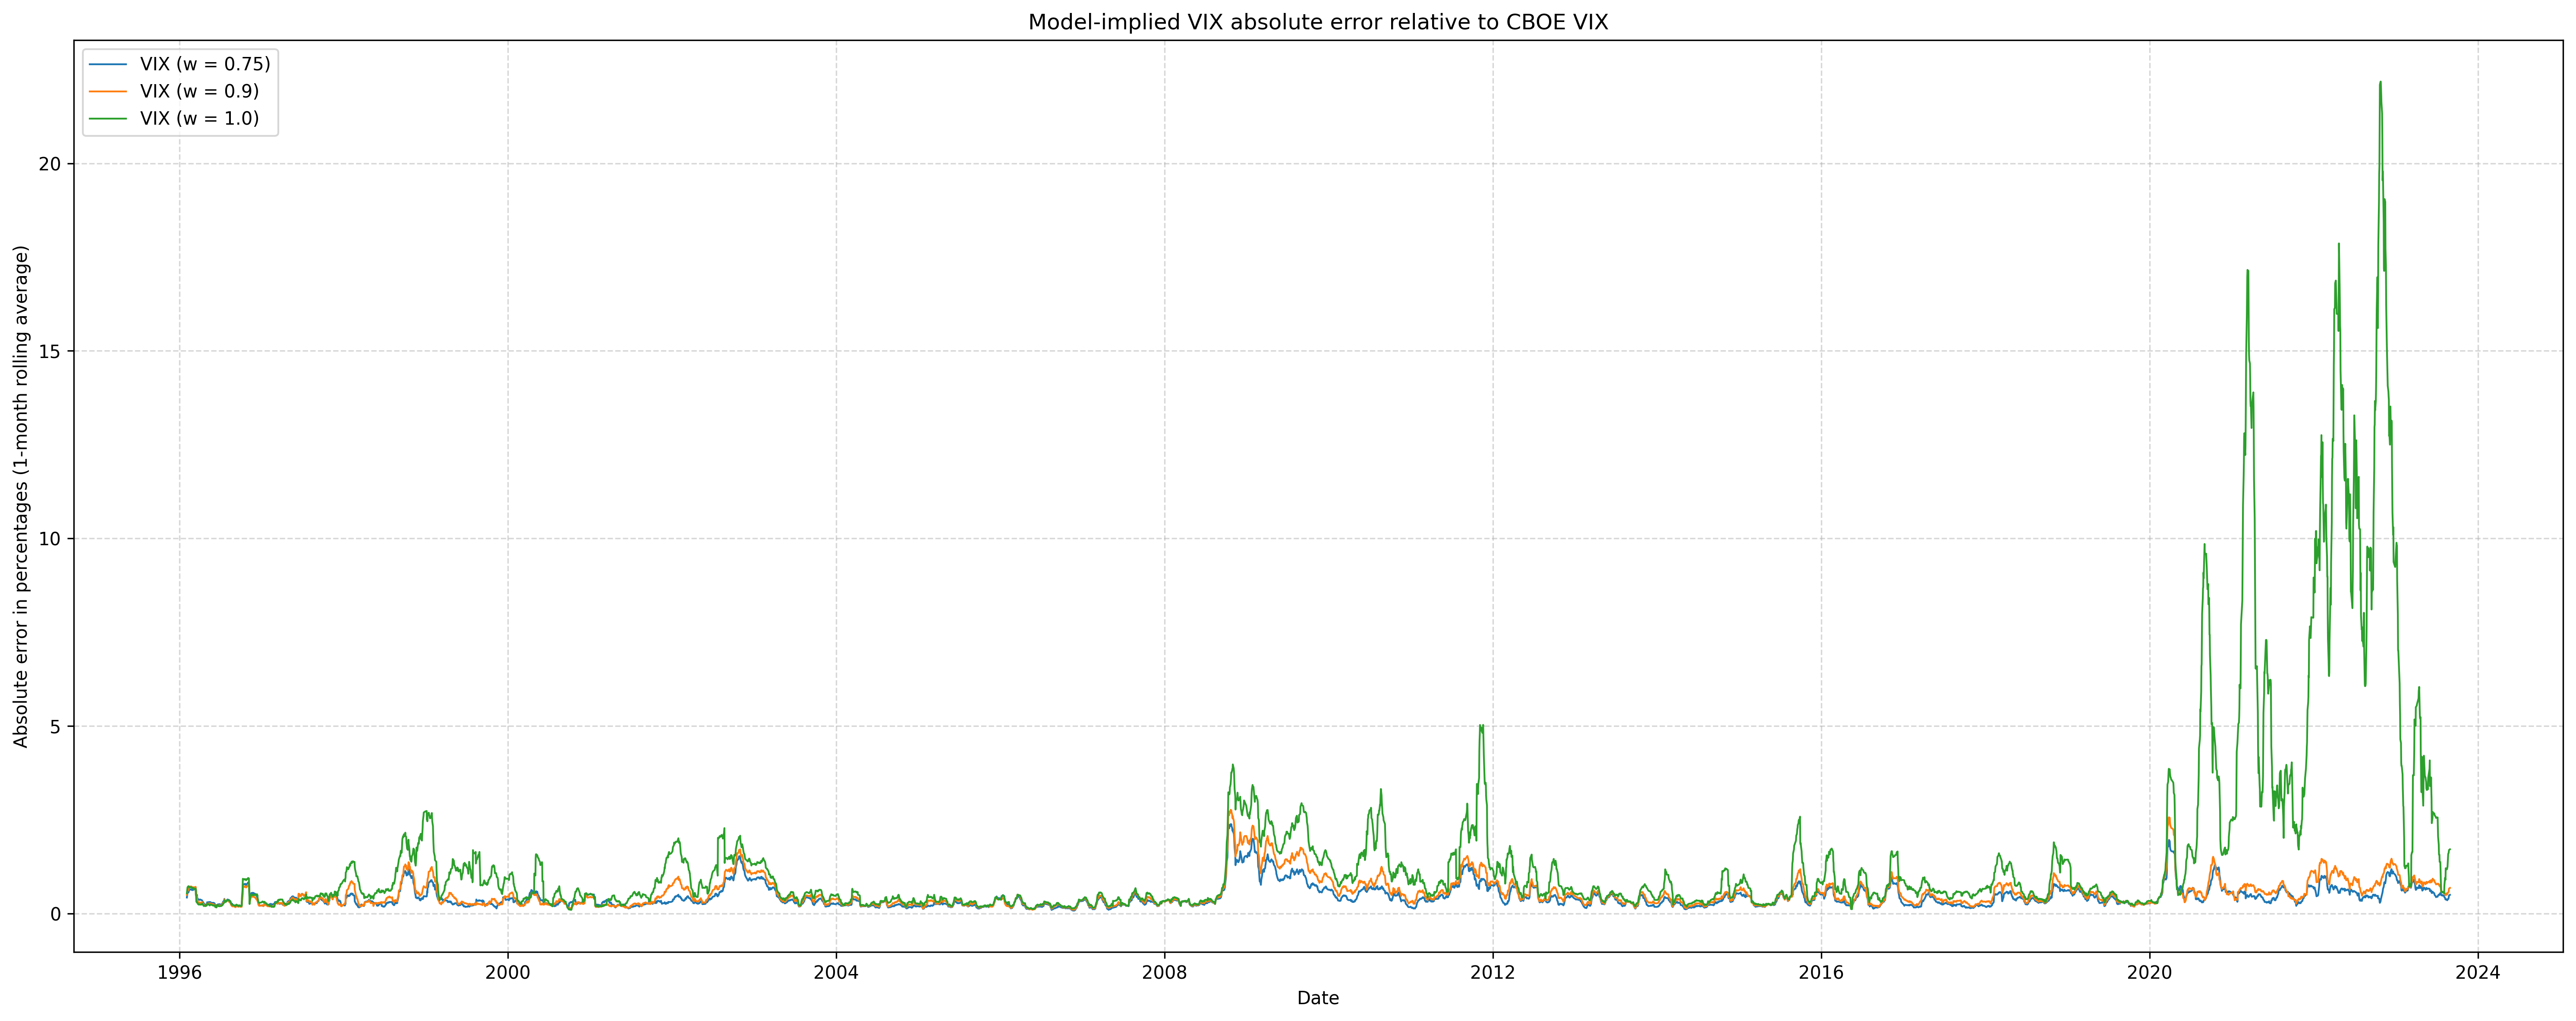
\includegraphics[width=1\linewidth]{figs/VIX_error.png}
    \caption{One-month moving average of absolute errors between model-implied one-month VIX from Bates models calibrated using $\alpha\in [0.75, 0.9, 1.0]$ and the VIX time series from CBOE. Errors for models calibrated using $\alpha$ hyperparameters equal to 0.75, 0.9, and 1.0 are in blue, orange, and green respectively. }
    \label{fig: VIX_alpha}
\end{figure}

The presence of a term penalizing deviations from a variance term structure is useful even when the model is mis-specified. This is because for values of $\alpha$ greater than zero, the error term for the variance term structure has a regularizing effect on calibrated model's implied variances. Figure \ref{fig: VIX_alpha} plots the absolute errors in the one-month $VIX$ for $\alpha \in \lbrace 0.75, 0.9, 1\rbrace$ implied by Bates models calibrated on my SPX panel relative to CBOE's published VIX. I find that the error is large in crises and becomes very large towards the end of my sample where the short-maturity segment of the SPX volatility surfaces is densely packed with short maturity weekly options. Using a value of $\alpha$ less than but close to 1, produces a time series of substantially lower errors.

 
\subsection{Exploring the significance of jumps}\label{subsec: SPX_jump_process}
Since the model can reproduce the term structure of the VIX with reasonable accuracy, I use it to examine the impact of jumps on expected variance, or equivalently the pricing of variance swaps. As discussed in section \ref{sec: theory}, the payoff of a variance swap is the realized variance of the underlying process with the fair value of this payoff being equal to the variance swap rate. \cite{ait2020term} use the gap between the VIX and the variance swap rate to examine the role of jumps in the overall price fluctuations of the S\&P 500. 

Recall from section \ref{sec: theory} that the magnitude of the spread reflects the skewness of the jump distribution. A positive spread indicates that the jump distribution is negatively skewed. On the right, figure \ref{fig:VIX_mult_spread} plots the one-month moving average of difference between the square root of the one-month maturity variance swap rate and the CBOE VIX implied by calibrated Bates models on SPX. The models were calibrated with the objective function from \eqref{eq: obj_function_special_case} with hyperparameter $\alpha = 0.9$. Note the spread is always positive, reflecting the well-known negatively skewed jump distribution of equity indices, with the spread widening during times of crisis. In figure \ref{fig:VIX_mult_spread}, the spread is particularly wide during the 2008-2009 financial crisis and the COVID pandemic era. 


A related quantity is the log contract multiplier of \cite{carr2012variance} and \cite{carr2021pricing} computed in \eqref{eq: multiplier}. A multiplier greater than 2 imply a negatively skewed jump distribution, with the difference between two quantifying the extent to which the jump distribution is skewed. On the left panel of figure \ref{fig:VIX_mult_spread}, I plot the one-month moving average time series of the log contract multiplier. The multiplier is persistently above 2, again consistent with the negatively skewed jump distribution of equity indices. In addition, how skewed the jump distribution appears to be time-varying consistent with the findings of \cite{ait2020term}, peaking around the crises associated with the onset of the second Iraq war, the 2008-2009 financial crisis, and the COVID pandemic. 

Overall, the calibration methodology produces a model which fits the term structure of variance well, facilitating analysis of the role of jumps in the expected volatility of the market. Both the variance swap spread relative to VIX and the log contract multiplier show persistent evidence of a negatively skewed jump distribution, with spreads and multipliers widening during crises. These measures highlight that the degree of skewness is time-varying, peaking during periods of high market stress.


\begin{figure}[!t]
    \centering
    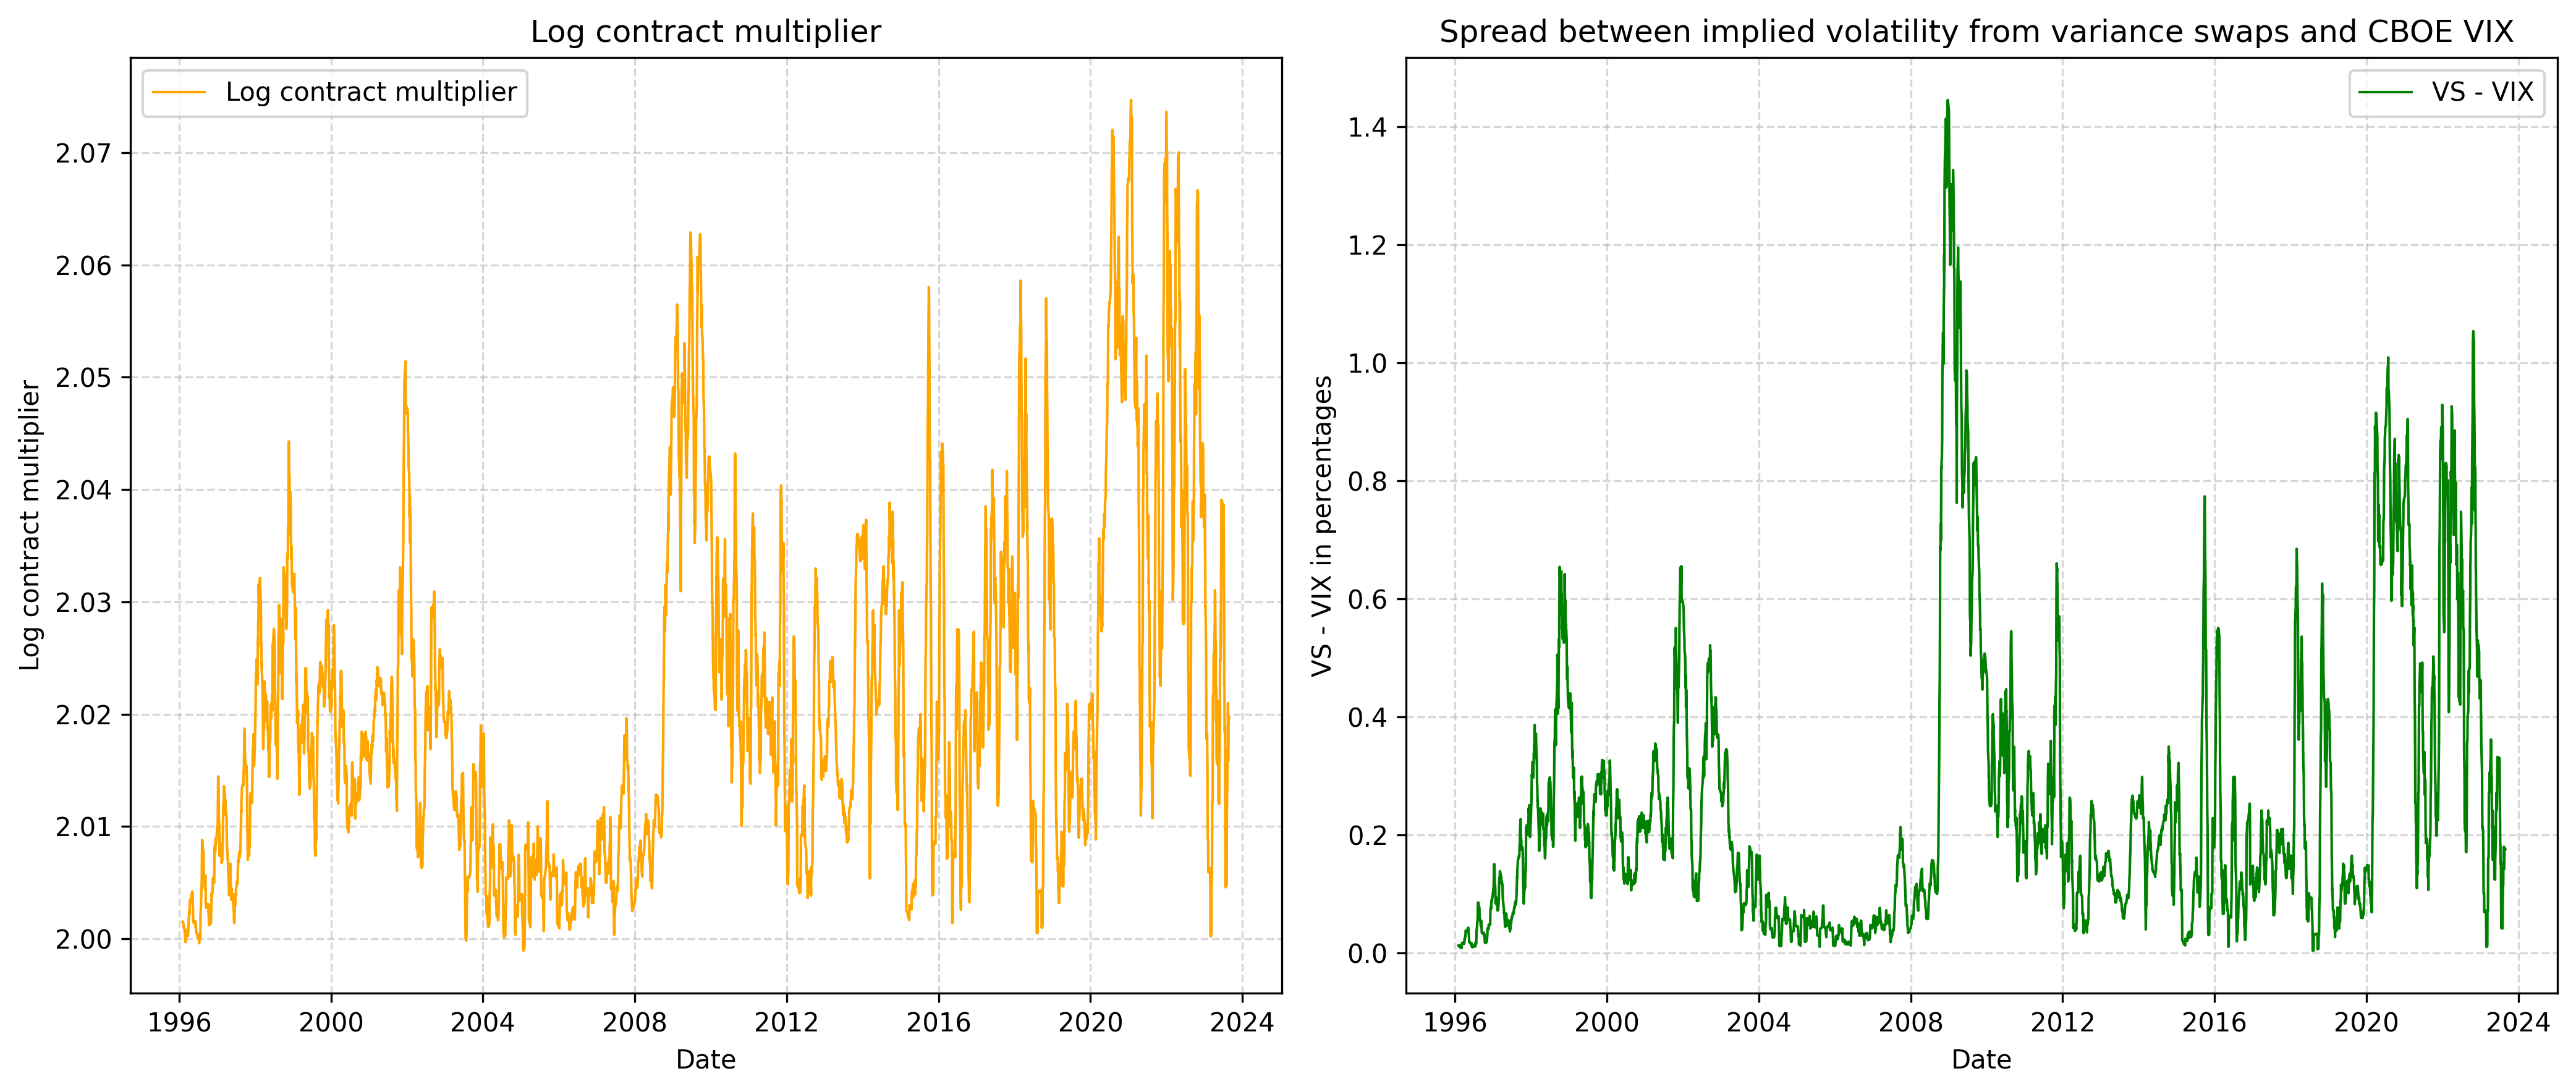
\includegraphics[width=1\linewidth]{figs/VS_minus_VIX.png}
    \caption{One-month moving average of log contract multiplier (left) computed using equation \eqref{eq: multiplier} and variance swap/VIX spread in implied volatility units (right). Quantities computed from for Bates models calibrated on the SPX volatility surface and VIX term structure with $\alpha = 0.9$.  }
    \label{fig:VIX_mult_spread}
\end{figure}


\section{Conclusion}\label{sec: conclusion}
The calibration of option pricing models is a routine procedure across both industry practice and academic research. This article offers a calibration procedure based on an objective function which jointly considers errors in the implied volatility surface and errors in the term structure of variance. My objective function can use either the term structure of variance swap rates or the VIX as an input. The ability to use the VIX is useful for a variety of underlying assets as many underlying assets with options do not have a corresponding variance swaps market and the VIX can be readily replicated from observed option prices. The error in the variance term structure is used as a regularization term for the objective function, akin to Tikhonov regularization penalty employed in ill-posed linear regression models. As I show in an empirical exercise, this discourages parameter values which imply unreasonable levels of future volatility. 

The hyperparameter $\alpha$ in this objective function governs the relative importance between fitting the variance term structure and the volatility surface. $\alpha$ ranges from 0 to 1, with higher values placing greater emphasis on fitting the volatility surface. To provide guidance on the choice of $\alpha$, I conduct calibration exercises using the S\&P 500 equity index option data and run simulations to examine the potential trade-offs between fit quality in the volatility surface and in the variance term structure. 

In practice, I find that a value around $\alpha = 0.9$ produces parameters which fit the volatility surface well and simultaneously implies option prices which can be reconciled with the variance term structure implied by the market. While there exists a trade-off between fitting the term structure of variance and the volatility surface, the numerical exercises in section \ref{sec: emp_results} suggest this trade-off is minimal for certain ranges for $\alpha$. For this reason, a value of $\alpha$ between 0.5 and 0.9 is recommended as in empirical settings provided an option pricing model of reasonable flexibility is chosen for calibration. 

\section{Appendix: Proofs}
\textit{Proof of proposition 1: } Since the market is free of arbitrage, the price of a time $T$ maturity swap, $VS(T; \lambda, J)$, for an underlying following a SJD process with jump size $J$ and jump intensity $\lambda$ is pinned down by the expectation of the quadratic variation as in \eqref{eq: QV} under the pricing measure. That is,
$$VS(T; \lambda, J) = \mathbb{E}\left[QV(\tau)\vert \lambda, J\right] = \mathbb{E}\left[ \int_0^{\tau} \left(d\log S_t\right)^2 =   \int_0^{\tau}  V_t d t + \int_0^{\tau}  \int_{\mathbb{R}} J^2 \nu(d s, d x)\Big\vert \lambda, J\right]$$
where $\mathbb{E}(\cdot\vert \lambda, J)$ is the expectation taken over the pricing measure induced by the jump parameters and the known diffusive volatility $\sigma$. The computation of the expectation of each integral in the sum is straightforward yielding:
$$VS(T; \lambda, J) =  \sigma^2  + \lambda J^2$$
Both $\lambda \neq 0$ and $J\neq 0$ by assumption, permitting rearrangement of the variance swap price which defines a relationship that must hold between the jump parameters:
$$\lambda =  \dfrac{ VS(T; \lambda, J) - \sigma^2}{J^2} $$
Since the variance swap is priced under the true parameters $\lambda^*$ and $J^*$, the function $\lambda(J)$ is observable:
$$\lambda(J) =  \dfrac{VS(T; \lambda^*, J^*) - \sigma^2}{J^2}$$
Therefore, we can substitute for $\lambda$ the expression above in the summation being minimized in \eqref{eq: prop_sjd_11}, converting the bivariate problem in \eqref{eq: prop_sjd_11} into the univariate problem in \eqref{eq: prop_sjd_12}. \qed \\
\\
\textit{Proof of proposition 2: } Since the market is free of arbitrage and OTM option prices are observed, $VIX^2(T; \lambda^*, J^*)$ is observable via static replication:
$$   VIX^2(T; \lambda^*, J^*) = \dfrac{2}{T}\left[\int_0^{S_0} \dfrac{P^{SJD}(K; \lambda^*, J^*)}{K^2} \, dK +  \int_{S_0}^\infty \dfrac{C^{SJD}(K; \lambda^*,J^*)}{K^2}  \, dK \right]$$
Equation \eqref{eq: VIX_gap} relates $VIX^2(T)$ to the variance swap price $VS(T)$ under the true parameters: 
$$ VS(T; \lambda^*, J^*) - VIX^2(T; \lambda^*, J^*)  = 2\lambda^*(1 + J^* - e^{J^*}) $$
Although we do not observe the variance swap price, we may write its no arbitrage price in terms of the unobserved jump parameters. Substituting the variance swap price from the proof of proposition 1, we have:
$$ \sigma^2 + \lambda J^2 - VIX^2(T; \lambda^*, J^*) = 2\lambda(1 + J - e^{J})$$
Rearranging yields an observable function $\lambda(J)$ which must hold in the absence of arbitrage:
$$\lambda =\dfrac{ VIX^2(T; \lambda^*, J^*)  - \sigma^2}{2(1+J - e^{J})} $$
Therefore, we can substitute for $\lambda$ the expression above in the summation being minimized in \eqref{eq: prop_sjd_21}, converting the bivariate problem in \eqref{eq: prop_sjd_21} into the univariate problem in \eqref{eq: prop_sjd_22}.
\qed \\ 
\\
\textit{Proof of proposition 3: } If the model is correctly specified, that is, the underlying price process follows the stochastic process in \eqref{eq: general_process_sde}, it is clear that $\Theta^*$ solves the minimization problem in \eqref{eq: general_opt}. This is holds as the minimum of any linear combination of squared terms with non-negative coefficients is attained at zero when $\Theta = \Theta^*$. For each term in the sum of \eqref{eq: general_opt} with non-negative weight $w_{i,j}$, we have:
$$w_{i,j}\left[\sigma(K_i, \tau_j; \Theta) - \sigma^{mkt}(K_i, \tau_j)\right]^2  = 0$$
for all $i,j$ when evaluated at $\Theta = \Theta^*$. Likewise, at $\Theta = \Theta^*$, $g^{VS}(\Theta) = 0$ and $g^{VIX}(\Theta) = 0$ for any non-negative constants $w^v_j$ by similar reasoning.

To show that the objective function is observable, first consider the objective in \eqref{eq: prop_general_opt} when $g(\Theta) = g^{VS}(\Theta)$ and variance swap rates are observed. It is clear that the sum of squared errors in contract implied volatilities is observable. The model-implied variance swap rates are observable given the parameter vector $\Theta$ by computing the following expectation of the quadratic variation:
$$VS(\tau_j; \Theta) = \mathbb{E}\left[QV(\tau_j) \vert \Theta\right] = \dfrac{1}{\tau} \mathbb{E}\left[\int_0^{\tau} V_t  d t + \int_0^{\tau} \int_{\mathbb{R}} J^2 \nu(d s, d x)\Big\vert \Theta\right ]$$
where $\mathbb{E}\left(\cdot\vert \Theta\right)$ is the expectation over the pricing measure induced by the parameter vector $\Theta$. Since market variance swap rates $VS^{mkt}(\tau_j)$ are observable, each term in the sum of $g^{VS}(\Theta)$ is observable:
$$w_j^v \left[VS(\tau_j;  \Theta) - VS^{mkt}(\tau_j)\right]^2 $$
Thus, both summations in the objective function below are observable and do not require the $S_t$ to be the true data generating process:.
$$\sum\limits_{j=1}^{M}\sum\limits_{i=1}^{N(\tau_j)} w_{i,j}\left[\sigma(K_i, \tau_j; \Theta) - \sigma^{mkt}(K_i, \tau_j)\right]^2 +  g^{VS}(\Theta) $$

To show that the objective function is observable when only option prices are observable, it suffices to show $g^{VIX}(\Theta)$ is observable since, as before, the sum of squared errors in contract implied volatilities is observable. Let $C^{mkt}(K, \tau)$ and $P^{mkt}(K, \tau)$ denote the market prices of put and call options with strike $K$ and time to maturity $\tau$. Since the market is free of arbitrage and OTM option prices are observed, $VIX^{mkt}(\tau_j)$ is recovered from market option prices via static replication:
$$  \left[VIX^{mkt}(\tau_j)\right]^2   = \dfrac{2}{\tau_j}\left[\int_0^{S_0} \dfrac{P^{mkt}(K, \tau_j)}{K^2} \, dK +  \int_{S_0}^\infty \dfrac{C^{mkt}(K, \tau_j)}{K^2}  \, dK \right]$$
for each $\tau_j \in \lbrace \tau_1, \ldots, \tau_M\rbrace$. Given the model parameter $\Theta$, which in turn specifies the product jump measure and variance process, the quantity $VIX^2(\tau_j; \Theta)$ can be computed from the stochastic differential equation of the underlying. As shown by \cite{ait2020term}, we can write the difference between the model-implied variance swap price and the model-implied VIX as follows:
$$VS(\tau_j; \Theta) - VIX^2(\tau_j; \Theta) = 2\lambda \mathbb{E}(1+J+J^2/2 - e^J\vert \Theta) $$
where $\lambda = \mathbb{E}\left[\int_0^{\tau_j} \lambda_t \, dt \vert \Theta\right]/\tau_j$. Since both $\mathbb{E}\left[QV(\tau_j) \vert \Theta\right]$ and $2\lambda \mathbb{E}(1+J+J^2/2 - e^J\vert \Theta)$ are computable from the model, $ VIX^2(\tau_j; \Theta)$ is observable. Therefore, $g^{VIX}(\Theta)$ is observable as each term in the summation in \eqref{eq: reg_term_VIX}:
$$w^v_j \left[VIX(\tau_j; \Theta) - VIX^{mkt}(\tau_j)\right]^2$$
is observable to the econometrician. Thus, the objective function below is observable whenever option prices are observed with the objective function being observable whether or not the variance swap term structure is observed.
$$\sum\limits_{j=1}^{M}\sum\limits_{i=1}^{N(\tau_j)} w_{i,j}\left[\sigma(K_i, \tau_j; \Theta) - \sigma^{mkt}(K_i, \tau_j)\right]^2 +  g^{VIX}(\Theta) $$ 
\qed 

\begin{comment}

\subsection{Proof of Proposition 3}
\textit{Proof: } I first compute the expectation of realized variance over the life of the option in the time interval $[0,T]$ at time $t = 0$. Let $\mathbb{Q}$ be the pricing measure associated with the Simple Jump Diffusion (SJD) with known diffusion parameter $\sigma$ and unobserved parameters $\lambda$ (jump intensity) and $J$ (jump size). I evaluate the quantity $QV(T)$ as defined in equation \eqref{eq: QV}, adapting the integrals for the SJD price process. Doing so we get
\begin{equation}\label{eq: app_1}
    QV(T)  = \int_0^T \left(d\log S_t\right)^2  =   \left(\int_0^T \sigma^2 dt + \int_0^T \int_{\mathbb{R}} J^2 \nu(\lambda, J)\right) 
\end{equation}
where $\nu(\lambda, J)$ is the product jump measure with $\lambda\delta_J$ as the Levy density of the price process.\footnote{$\delta_a(X)$ denotes the Dirac measure for $a\in \mathbb{R}$ that is equal 1 if $a\in X$ and 0 otherwise. }
The first term in the sum is the component of expected variance associated with the diffusion term while the second sum is the portion of expected variance associated with the jump process. Taking expectations and evaluating the integrals in \eqref{eq: app_1} we get:
\begin{equation}\label{eq: app_1}
   V(T) =  \mathbb{E}^\mathbb{Q}\left[\int_0^T \left(d\log S_t\right)^2 \right] =  \mathbb{E}^\mathbb{Q}\left[ \int_0^T \sigma^2 d t + \int_0^T \int_{\mathbb{R}} J^2 \nu(\lambda, J)\right]  =  \sigma^2 T+\lambda T J^2
\end{equation}
I apply the main theoretical result of \cite{carr2012variance}; for completeness, I state this below. 

\begin{proposition}\label{prop: carrwu} \citep{carr2012variance} Let $X_t$ be a Levy process with Brownian variance $\sigma^2$ and Levy measure $\nu$. Let $\mathbb{E}$ be the time $0$ expectation operator for the filtered probability space $(\Omega, (\mathcal{F}_u)_{u\geq 0}, \mathbb{P})$ satisfying the usual conditions \citep{protter2004stochastic}. Fix $T > 0$; the expected variance from time $0$ to $T$ can be expressed as a multiple of the price of a contract paying the logarithm of gross return $X_T/X_0$:
\begin{equation}\label{eq:app2}
\mathbb{E} \left[\int_0^T \left(d\log S_t\right)^2 \right]  = \mathbb{E} \left[\int_0^T \sigma^2 \, dt \right] + \mathbb{E} \left[\int_0^T\int_\mathbb{R} J^2 \, d\nu(J) \right] = Q_X\mathbb{E}\left[-\log\left(\dfrac{X_T}{X_0}\right)\right] 
\end{equation}
The multiplier $Q_X$ itself can be defined in terms of the cumulant generating function. Let $\kappa_X(u) =\log\mathbb{E}(e^{uX_T})$ denote the cumulant-generating function of $X_T$. The multiplier $Q_X$ is given by: 
\begin{equation}\label{eq:app3}
Q_X = \frac{\kappa_X^{\prime \prime}(0)}{\kappa_X(1)-\kappa_X^{\prime}(0)}
\end{equation}
\qed
\end{proposition}
We can apply proposition \eqref{carrwu_prop} to the SJD process. The SJD price process is a Levy process with Brownian variance $\sigma^2$ and Levy measure $\lambda \delta_J(x)$ where $\delta_J(A)$ the Dirac measure that is 1 if $J\in A$ and zero otherwise. I evaluate the necessary values of the cumulant-generating function and its derivatives and substitute them into equation \eqref{eq:app3}. Doing this and simplifying, I obtain the following expression for the multiplier associated with the SJD process with jump size $J$ and jump intensity $\lambda$:
\begin{equation}\label{eq:app_mult}
    Q^{SJD} = \dfrac{ \sigma^2  +  \lambda J^2}{\sigma^2 + \lambda(e^J - 1 - J)}
\end{equation}
Plugging in $Q^{SJD}$ as the multiplier in \eqref{eq:app3}, we have
$$ \dfrac{ \sigma^2 +  \lambda J^2}{\sigma^2 + \lambda(e^J - 1 - J)} \mathbb{E}\left[-\log\left(\dfrac{X_T}{X_0}\right)\right]  =  \mathbb{E}\left[ QV(T) \right] = \sigma^2 T  +\lambda T   J^2.$$
It is well-known that the log return in the expectation can be readily replicated by a static portfolio of options. The replication is immediate from the \cite{carr2001optimal} formula:
\begin{equation}\label{eq:app_log}
    \mathbb{E}\left[-2\log\left(\dfrac{X_T}{X_0}\right)\right] = 2\int_0^\infty \dfrac{P(K,T)}{K^2} \, dK 
\end{equation}
where $P(K,T)$ is the price of an out-of-the-money option with maturity $T$ and strike price $K$. Substituting \eqref{eq:app_log} into \eqref{eq:app_mult} and simplifying yields
\begin{equation}\label{eq:app_11}
  2 \int_0^\infty \dfrac{P(K,T)}{K^2} \, dK = \sigma^2 T + \lambda T(e^J - 1 - J) = \sigma^2 T + \lambda T \left( \dfrac{J^2}{2!} +  \dfrac{J^3}{3!} + \ldots\right)
\end{equation}
where the final equality applies the power series expansion for Euler's function. Define $V(T)$ to be the expected quadratic variation over the life of the option. By direct computation, I can write
\begin{equation}\label{eq:app_12}
  2 \int_0^\infty \dfrac{P(K,T)}{K^2} \, dK   = \sigma^2 T +2 \lambda T \left( \dfrac{J^2}{2!} +  \dfrac{J^3}{3!} + \ldots\right) = V(T)  + 2\lambda T\left(\dfrac{J^3}{3!} + \dfrac{J^4}{4!}+ \ldots\right)
\end{equation}
The above expression shows that a VIX-like computation (the left-hand side integral) does not exactly recover the expected quadratic variation in the presence of jumps. Note that without jumps ($\lambda = 0$ and/or $J = 0$), we recover the standard result of \cite{neuberger1994log} which identifies the expected quadratic variation of a pure diffusion process by computing the integral in \eqref{eq:app_12}. As noted by \cite{jiang2005model}, the VIX recovers the model-free variance only in an approximate sense - the square of the VIX is equal to the expected quadratic variation plus a summation consisting of higher-order moments of the jump distribution. Rearranging equation \eqref{eq:app_12}, I obtain
\begin{equation}\label{eq:app_13}
  V(T) - 2 \int_0^\infty \dfrac{P(K,T)}{K^2} \, dK - 2\lambda T \sum\limits_{k=3}^\infty \dfrac{J^k}{k!} = 0
\end{equation}
which verifies equation \eqref{eq:sys_ts}. Equation \eqref{eq:sys_ivs} holds since the market prices were generated under the SJD model.  \qed


\subsection{Proof of Proposition 2}
\textit{Proof: } Using a version of Ito's lemma for jump processes, I first obtain the stochastic differential equation (SDE) for the log price:
\begin{equation}\label{eq:app4}
    d\log(S_t) = -\dfrac{V_t}{2} \, dt + \sqrt{V_t} dW_t + J_t dN_t - \lambda\mathbb{E}^\mathbb{Q}_t\left[ e^{J_t} - 1\right] \, dt 
\end{equation}
Using SDE in \eqref{eq:app4}, I compute the risk-neutral expectation of the log return $\log S_T/S_0$. Integrating \eqref{eq:app4}, 
\begin{equation}\label{eq:app5}
    \mathbb{E}\left[-\log\left( \dfrac{S_\tau}{S_0} \right)\right] = -\mathbb{E} \left[\int_0^\tau d\log S_t  \right] = \dfrac{1}{2} \int_{0}^{\tau} V_t \, dt + \lambda\tau\mathbb{E}\left[e^{J_t} - 1 - J_t\right].
\end{equation}
The expected annualized quadratic variance is given by:
\begin{equation}
   \dfrac{1}{\tau}\mathbb{E}\left[QV(\tau)\right] = \dfrac{1}{\tau} \int_{0}^{\tau} V_t \, dt + \lambda\mathbb{E}\left[J^2_t\right]
\end{equation}
By direct substitution, one can verify that
\begin{equation}\label{eq:app21}
     \dfrac{1}{\tau}\mathbb{E}\left[QV(\tau)\right]  -   \dfrac{2}{\tau}\mathbb{E}\left[\log\left( \dfrac{S_\tau}{S_0} \right)\right]  = 2\lambda\mathbb{E}\left(1 + J_t + \dfrac{J_t^2}{2} - e^{J_t}\right)
\end{equation}


Substituting the third degree Taylor approximation polynomial of Euler's function into \eqref{eq:app21}, I can obtain the following:
\begin{equation}\label{eq:app21}
      \dfrac{1}{\tau}\mathbb{E}\left[QV(\tau)\right]-   \dfrac{2}{\tau}\mathbb{E}\left[\log\left( \dfrac{S_\tau}{S_0} \right)\right]   \approx -\lambda\mathbb{E}\left(\dfrac{J^3}{3}\right)
\end{equation}
\qed


\section{Appendix: Option pricing models}
I explore the use of three workhorse option pricing models in the literature: the jump-diffusion model of \cite{merton1976option} (MJD), the \cite{heston1993closed} stochastic volatility model, and the \cite{bates1996jumps} model which nests the prior two as special cases.  For what follows, let $S_t$ and $q$ denote the spot price of the underlying asset and its dividend yield. I use $r$ to denote the instantaneous risk-free return.

\subsection{Merton jump diffusion model}
The MJD model augments the diffusion process underlying the classic \cite{black1973pricing} model with lognormally distributed jumps. The jump arrivals are modeled as a Poisson process. Let $W^1_t$ be a Brownian motion. The dynamics of the MJD model are given by:
\begin{equation}
\begin{aligned}
& d S_t=\left(r-q-\lambda \mu_J\right) S_t d t+\sigma S_t d W_t^1+J S_t d N_t \\
& \mathbb{P}\left(d N_t=1\right)=\lambda  d t\\
& \ln (1+J) \sim N\left(\ln \left(1+\mu_J\right)-\frac{\sigma_J^2}{2}, \sigma_J^2 \right)
\end{aligned}
\end{equation}
The MJD model is pinned down by 4 parameters: the diffusion coefficient $\sigma$ and three parameters relating to the jump process. Jointly, the mean jump size $\mu_J$, its standard deviation $\sigma_J$, and Poisson jump intensity $\lambda$, govern the jump dynamics of the stochastic process. One technical complication with the MJD model is that the risk-neutral martingale measure $\mathbb{Q}$ is not unique, a property shared by many jump-diffusion models \citep{cont2003financial}. In fact, given a set of model parameters $(\sigma, \mu_J, \sigma_J, \lambda)$ is straightforward to generate model parameters which produce nearly identical pricing implications for conventional option maturities and strikes scaling the jump process parameters. The model parameters $(\sigma, \mu_J', \sigma_J', \lambda')$ defined by:
$$\mu_J' = c\mu_J \qquad \sigma_J' = c\sigma_J \qquad \lambda' = \lambda/c \qquad\qquad c\in (0,1)$$
imply a pricing measure with very similar option prices to the original parameters.



\subsection{Heston stochastic volatility model}
The Heston model features a bivariate diffusion process; one diffusion corresponds to the spot price of the underlying and the other governing the evolution of the variance process. The variance process is the familiar square root-process from the \cite{cox1985theory}. Let $W^1_t$ and $W^2_t$ denote Brownian motions. The dynamics of the Heston model are given by:
\begin{equation}
\begin{aligned}
& d S_t=\left(r-q\right) S_t d t+\sqrt{V_t} S_t d W_t  \\
& d V_t=\kappa\left(\theta-V_t\right) d t+\sigma_V \sqrt{V_t} d W_t^v \\
& \mathbb{E}\left[d W_t^1 d W_t^2\right]= \rho d t \\
\end{aligned}
\end{equation}
The model is pinned down by five parameters: $\rho$ determines the correlation between the two Brownian motions while other four define the spot variance process $V_t$. $V_0$ is the initial level of spot variance. $\theta$ is the long-run mean of the variance process while $\kappa$ governs the speed of mean revision. Lastly, the $\sigma^V$ is the volatility of the variance process.



The VIX formula of \cite{neuberger1994log} and \cite{jiang2005model} is based on a static replication of a particular payoff, namely the so-called "log contract". Following \cite{carr2012variance}, I define the log contract of maturity $\tau$ to be the payoff equal to negative one multiplied by the natural logarithm of the underlying return from time $t$ to $t + \tau$. 
\begin{equation}\label{eq: log_cont}
\mathbb{E}^\mathbb{Q}\left[ -\log\left(\dfrac{S_{t+\tau}}{S_t}\right) \right] = \int_{0}^{F_t} \dfrac{P_t(K,\tau)}{K^2}\, dK + \int_{F_t}^{\infty} \dfrac{C_t(K,\tau)}{K^2}\, dK
\end{equation}
In 2003, CBOE implemented a discretized variant of the formula above with the square of the VIX Index, stepping away from the prior approach based at-the-money implied volatilities on OEX (CBOE S\&P 100 Index) options. This formula remains in use, computing the square of the VIX as twice quantity in \eqref{eq: log_cont} using a thirty day horizon $(\tau = 30/365)$ as shown in equation \eqref{eq: VIX_cont_CBOE}:
\begin{equation}\label{eq: VIX_cont_CBOE}
    VIX^2 = \dfrac{365}{30} \left[\int_{0}^{F_t} \dfrac{P_t(K,\tau)}{K^2}\, dK + \int_{F_t}^{\infty} \dfrac{C_t(K,\tau)}{K^2}\, dK \right]
\end{equation}

(equivalently variance swap fair strikes) for maturity $\tau$ is given by:
\begin{equation}\label{eq:bates_mult}
\lambda \left[1 + \log(1 + \mu_J)-\sigma^2_J/2 + \frac{1}{2}\left[\log(1 + \mu_J) - \sigma^2_J/2\right]^2+ \sigma^2_J/2 - (1+\mu_J)\right] = 
\end{equation}
$$2\lambda \left[\log(1 + \mu_J) - \mu_J + \frac{1}{2}\left[\log(1 + \mu_J) - \sigma^2_J/2\right]^2  \right] $$
We can apply the well-known log approximation $\log(1+x) \approx x$ for small $x$. Doing so, we obtain the following expression:
$$2\lambda \left[\frac{1}{2}\left[\mu_J - \sigma^2_J/2\right]^2  \right] $$
    
\end{comment}



\begin{comment}

    \textbf{Deterministic basis surface theorem}\\
Denote the futures price of an asset with maturity $\tau$ by $F_t(\tau)$ and $C^{\tau}(K, T)$ to be the time $t$ price of a European-style call option with strike price $K$ and expiration $T$ written on the futures contract with maturity $\tau$. If $r_t$ is a predictable short rate process and there exists a unique risk-neutral pricing measure $\mathbb{Q}$, then for any two maturities $\tau_1$ and $\tau_2$ such that $t \leq \tau_1 < \tau_2$,
\\
\textit{Proof: Deterministic basis surface theorem}\\
Integrating the call payoff over the pricing measure $\mathbb{Q}$ (appropriately discounted) gives the call price:
\begin{equation}
    C^\tau(K,T) = DF(t, T)\displaystyle\int_0^\infty \max\lbrace F_T(\tau) - K, 0\rbrace \, d\mathbb{Q}
\end{equation}
where the discount factor $DF(t, T)$ is defined as:
$$    DF(t, T)= \dfrac{1}{T-t}\displaystyle\int_t^T  r_t\, dt $$
integral of $r_t$ from $t$ to $T$. \\
If interest rate process $r_t$ be predictable, then forward prices and futures prices coincide. This implies for all $\tau \geq T$,
\begin{equation}
    F_t(\tau) = e^{- DF(t, T)(\tau -T)} S_t 
\end{equation}
Substituting the forward price in for $F_t(\tau_2)$ yields
\begin{equation}\label{eq: app_call_price}
    C^{\tau_2}(K,T) =  DF(t, T)\displaystyle\int_0^\infty \max\lbrace e^{-DF(t, T)(\tau_2 -T)} S_t - K, 0\rbrace \, d\mathbb{Q}
\end{equation}
Note that 
\begin{align*}
e^{-DF(t, T)(\tau_2 -T)} S_t - K 
&=  e^{-DF(t, T)(\tau_2 -\tau_1)} \left[ e^{-DF(t, T)(\tau_1 -T)} S_t - e^{-DF(t, T)(\tau_2 - \tau_1)}K \right] \\
&=  e^{-DF(t, T)(\tau_2 -\tau_1)} \left[ F(\tau_1)  - e^{-DF(t, T)(\tau_2 - \tau_1)}K \right] 
\end{align*}
Substituting the third line into the integral in \eqref{eq: app_call_price} gives
\begin{equation}\label{eq: app_call_price2}
    C^{\tau_2}(K,T) = e^{-DF(t, T)(T-t)} \left( e^{-DF(t, T)(\tau_2 -\tau_1)} \displaystyle\int_0^\infty \max\lbrace  F(\tau_1)  - e^{-DF(t, T)(\tau_2 - \tau_1)}K   , 0\rbrace \, d\mathbb{Q}\right)
\end{equation}
Note the expression between parentheses in equation \eqref{eq: app_call_price2} is the price of exactly $e^{-DF(t, T)(\tau_2 -\tau_1)}$ units of a call option with the same maturity $T$ and strike price $K$ but written on the futures contract maturing at $\tau_1$. Equivalently, we may write
\begin{equation}\label{eq: app_call_price3}
    C^{\tau_2}(K,T) = e^{-DF(t, T)(T-t)}  C^{\tau_1}(K,T) 
\end{equation}
Note that if $\tau_1 = T$, this is equivalent to a option written on the spot market. 

\end{comment}

\begin{comment}
    \section{Jump and diffusion risks}
Each of the three models sheds light on the sources of variation in the underlying. All three models share a diffusive risk component, while the MJD and Bates models also admit jumps. For each of these models, we can compute a measure similar in spirit to the VIX: the model implied risk-neutral expected variance. Since the Bates model nests both the Heston and MJD model, I give the formula for the integrated variance observed from time $0$ to time $\tau$ for the general Bates model:
\begin{equation}
    \mathbb{E}^\mathbb{Q}\left(\dfrac{1}{\tau}\int_0^\tau V_t \, dt\right) =\theta+\frac{v_0-\theta}{\kappa T}\left(1-e^{-\kappa \tau}\right)+\lambda\left(\alpha^2+\sigma_J^2\right)
\end{equation}
where $\alpha = \ln(1+\mu_J) - \sigma^2_J/2$. Figures \ref{fig:IV2} and \ref{fig:IV3} shows the time series of this measure from 1996 to 2023 for our three pricing models. Figure \ref{fig:IV2} makes the calibration problem for the Bates model readily identifiable. Dates where it is far above the MJD integrated variance is suggestive of some faulty calibration.

\begin{table}[!t]
    \centering
\begin{tabular}{lrr}
\toprule
 & MJD & Hes \\
Event &  &  \\
\midrule
CPI MoM & 0.245366 & 0.185723 \\
Change in Nonfarm Payrolls & 0.239317 & 0.180272 \\
FOMC Rate Decision (Upper Bound) & 0.251103 & 0.213751 \\
GDP Annualized QoQ & 0.246983 & 0.194939 \\
ISM Manufacturing & 0.242512 & 0.192026 \\
ISM Services Index & 0.225646 & 0.157793 \\
PPI MoM & 0.262221 & 0.209528 \\
Unemployment Rate & 0.239317 & 0.180272 \\
None & 0.250916 & 0.190830 \\
\bottomrule
\end{tabular}
    \caption{Caption}
    \label{tab:my_label}
\end{table}


\section{Event risks}
To estimate announcement-related risks, use modified version of \cite{bates1991crash} model as in \cite{johannes2024expected}. The modified model assumes log of underlying evolves under the $\mathbb{Q}$-measure as follows:
$$
\begin{aligned}
d \log(S_t) & =\left(r-\frac{1}{2} v_t-\lambda\left(\mu_1-1\right)\right) d t+\sqrt{v_t} d W_{1 t}^{\mathbb{Q}}+d\left(\sum_{j=1}^{N_t^{\mathbb{Q}}} Y_j^{\mathbb{Q}}\right) + d\left(\sum_{j=1}^{M_t} Z_j^{\mathbb{Q}}\right)\\
d v_t & =\kappa\left(\theta-v_t\right) d t+\sigma_v \sqrt{v_t} d W_{2, t}^{\mathbb{Q}}
\end{aligned}
$$
where $\mu_y^{\mathbb{Q}}$ is the mean of the jump size $Y_j^{\mathbb{Q}} \sim \mathcal{N}\left(\mu_y^{\mathbb{Q}},\left(\sigma_y^{\mathbb{Q}}\right)^2\right), \lambda^{\mathbb{Q}}$ is the $N_t^{\mathbb{Q}}$ intensity, and the Brownian motions are correlated. \\

Option pricing is done using the characteristic function approach of \cite{carr1999option}.For the Bates model above, the characteristic function can be written analytically:
$$
\Psi_x(t, T, u)=e^{\alpha(t, T, u)+\beta(t, T, u) v_t+u x_t}
$$
where the coefficients $\beta(t, T, u)$ and $\alpha(t, T, u)$ are functions of the model parameters and time, and $u \in \mathbb{C}$. Using a calibrated Bates model we should be able to answer questions about variance risk premia, jump risk, and crash risks across a variety of assets that received weekly expirations. Equity indices are one - but many popular ETFs that cover various asset classes did as well (oil, natural gas, gold, sliver, treasuries). 

Total quadratic variation for a price process is given by 
$$Q V_t\equiv \frac{1}{T-t}  \int_t^T \sigma_s^2 d s +\frac{1}{T-t}  \int_t^T \int_{\mathbb{R}} x^2 \mu(d s, d x)$$
where $\mu(d s, d x)$ is the jump measure. From the calibrated model we could compute variance risk premium:
$$\mathbb{E}_t^\mathbb{P}(Q V_{t+1} ) - \mathbb{E}_t^\mathbb{Q}(Q V_{t+1}) $$

Crash risks can be computed from deep OTM call and put options as in \cite{bollerslev2011tails}. For jump risk, we can use the extracted risk-neutral parameters from the model, $\mu_y^{\mathbb{Q}}$ and $\left(\sigma_y^{\mathbb{Q}}\right)^2$.
 
\end{comment}

\bibliography{joint_calibration}
\end{document}